\onecolumn
\newpage

\section{Weighted least squares linear fits to Radon trace profiles}
\label{sec:WLS-fits}

\begin{figure*}
    \centering
    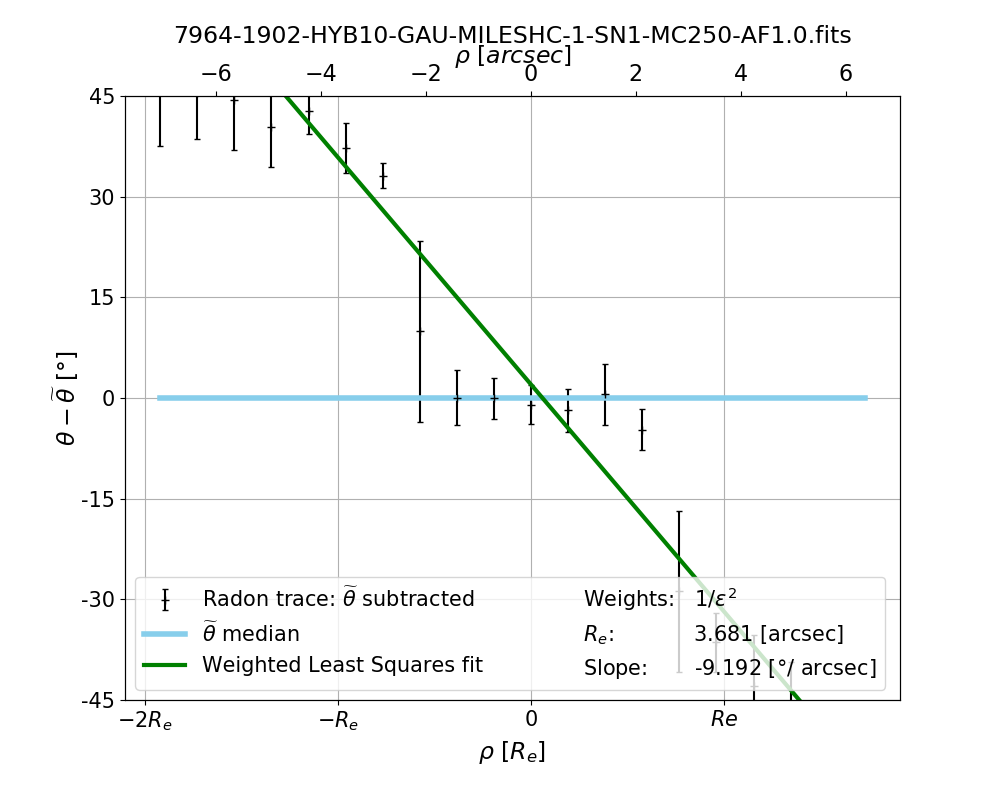
\includegraphics[width=0.31\textwidth]{Images/WLSFITS/CPSB/7964-1902.png}
    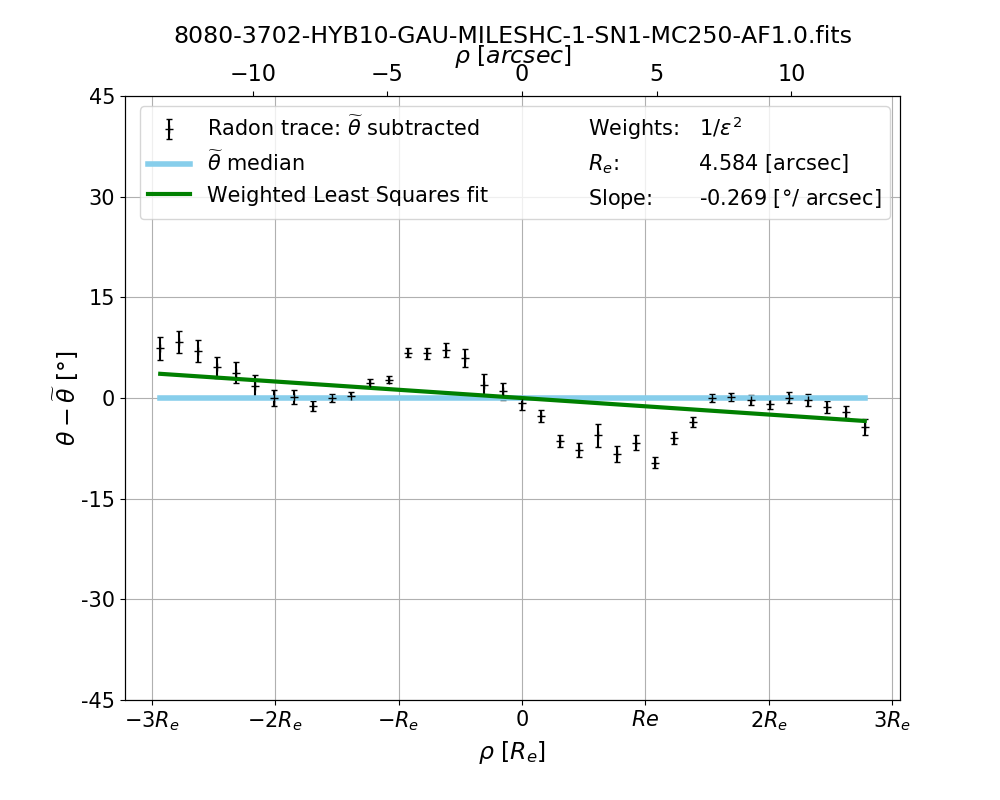
\includegraphics[width=0.31\textwidth]{Images/WLSFITS/CPSB/8080-3702.png}
    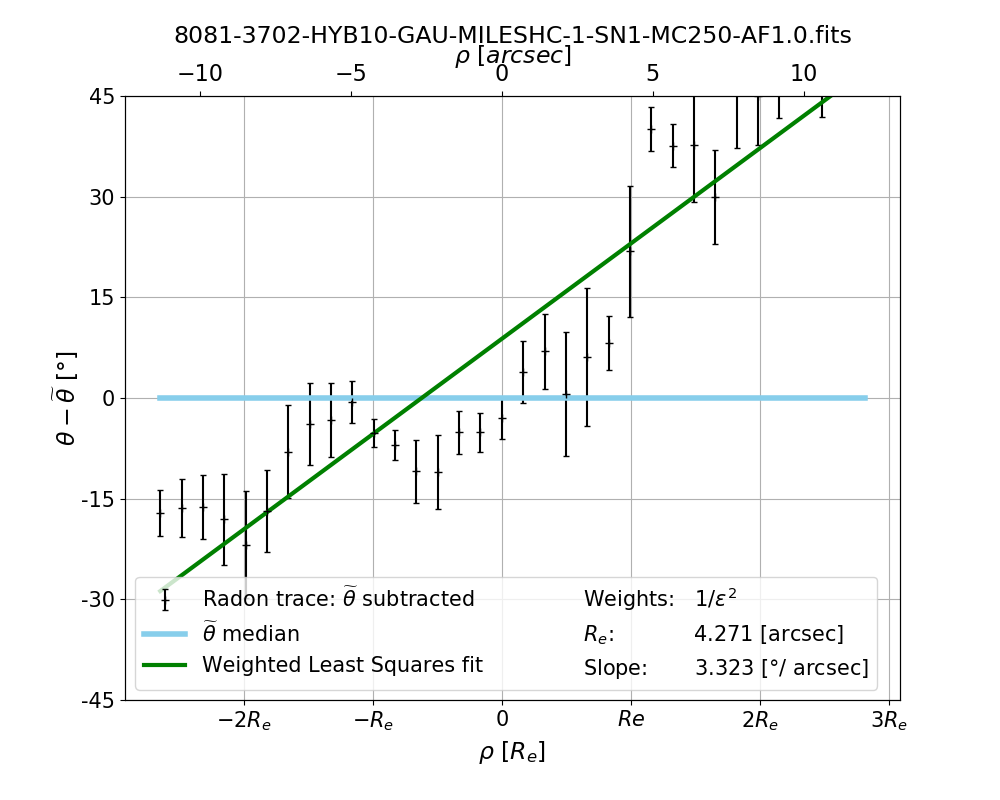
\includegraphics[width=0.31\textwidth]{Images/WLSFITS/CPSB/8081-3702.png}
    %
    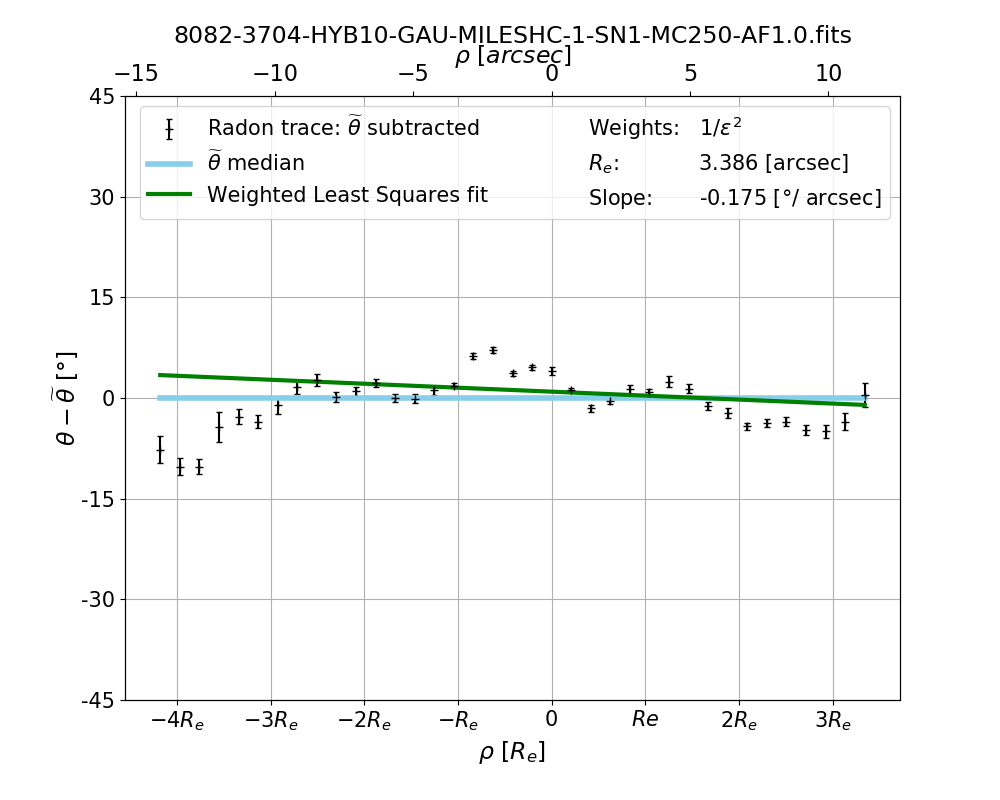
\includegraphics[width=0.31\textwidth]{Images/WLSFITS/CPSB/8082-3704.png}
    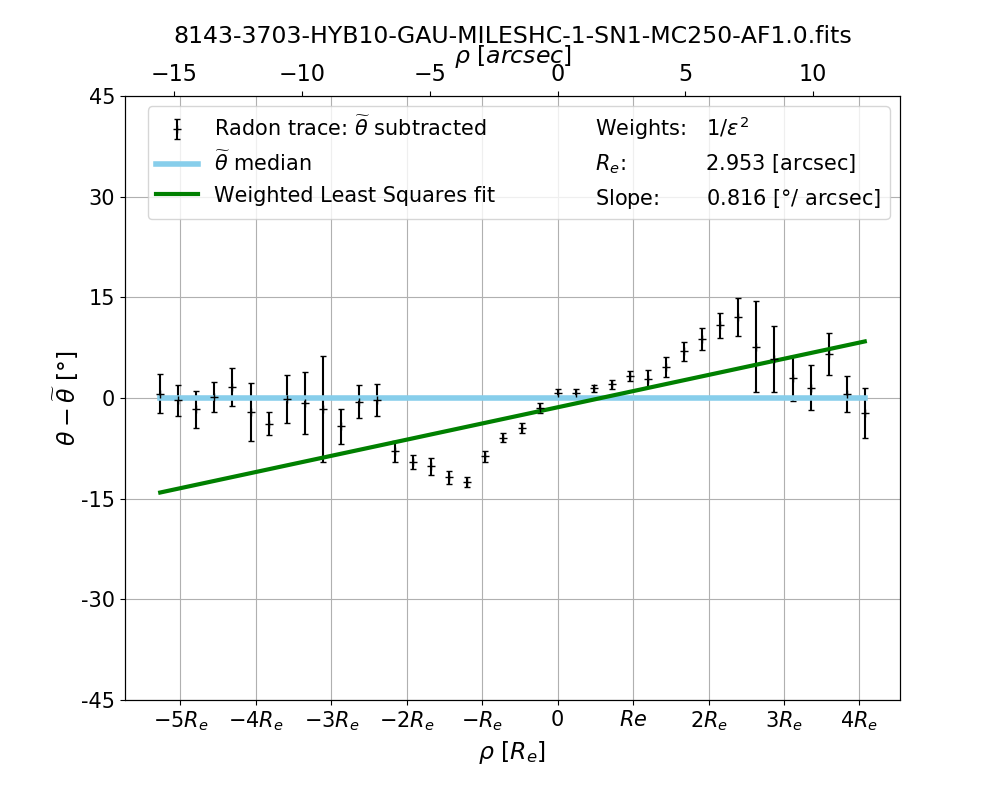
\includegraphics[width=0.31\textwidth]{Images/WLSFITS/CPSB/8143-3703.png}
    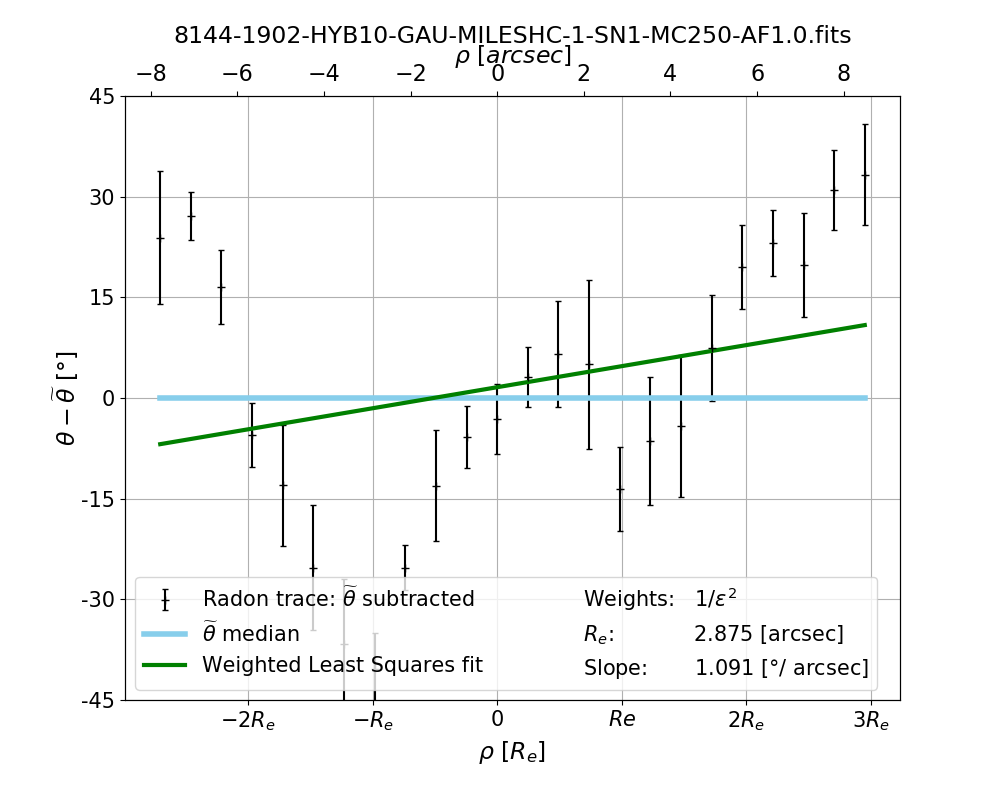
\includegraphics[width=0.31\textwidth]{Images/WLSFITS/CPSB/8144-1902.png}
    %
    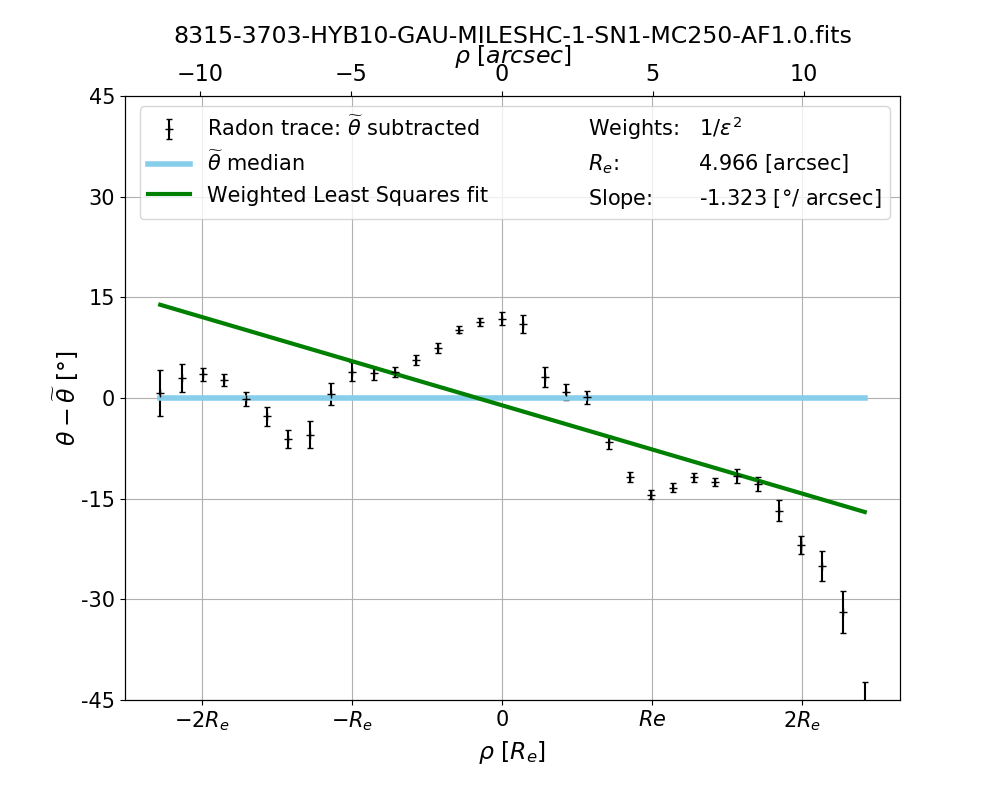
\includegraphics[width=0.31\textwidth]{Images/WLSFITS/CPSB/8315-3703.png}
    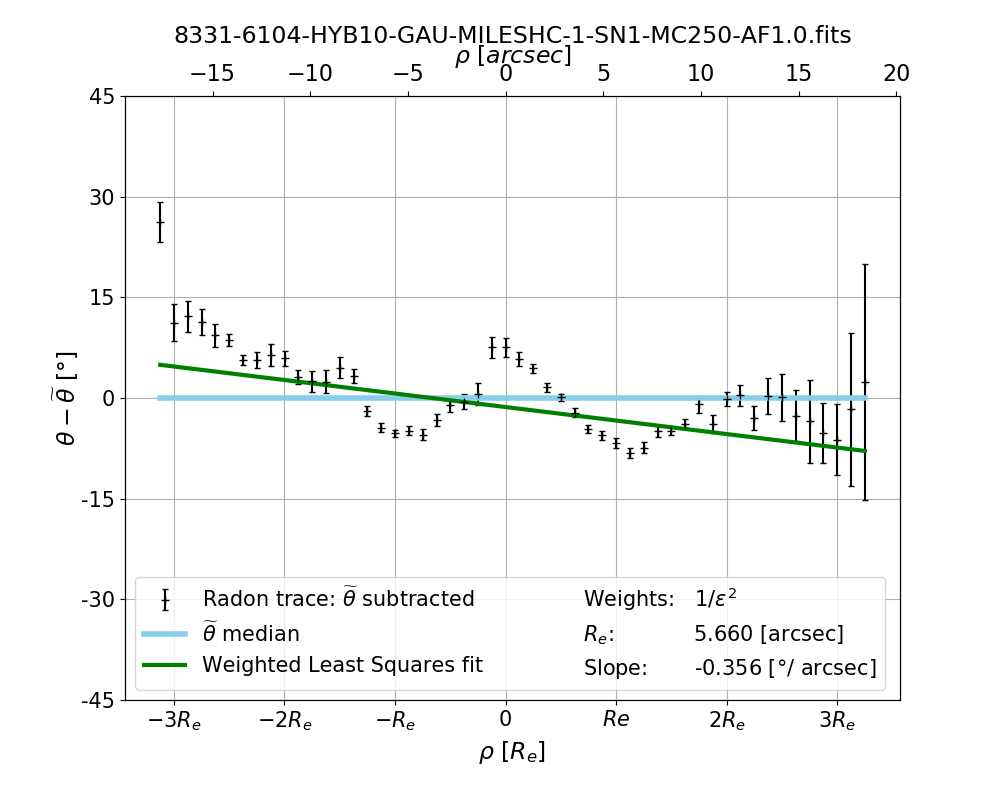
\includegraphics[width=0.31\textwidth]{Images/WLSFITS/CPSB/8331-6104.png}
    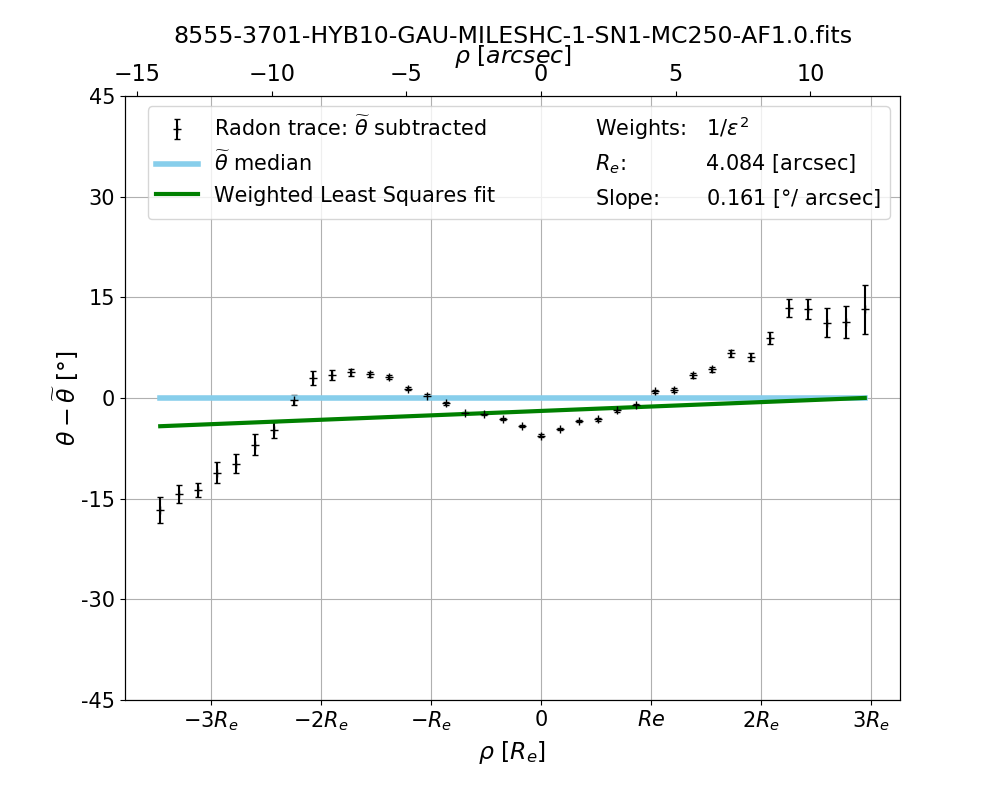
\includegraphics[width=0.31\textwidth]{Images/WLSFITS/CPSB/8555-3701.png}
    %
    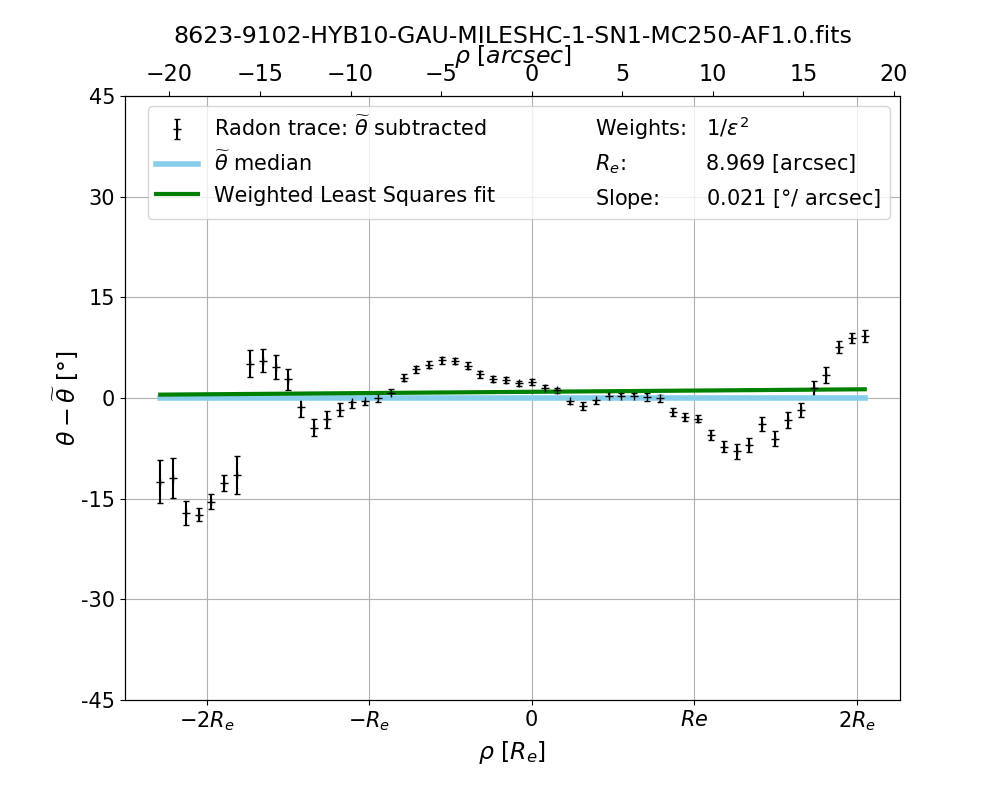
\includegraphics[width=0.31\textwidth]{Images/WLSFITS/CPSB/8623-9102.png}
    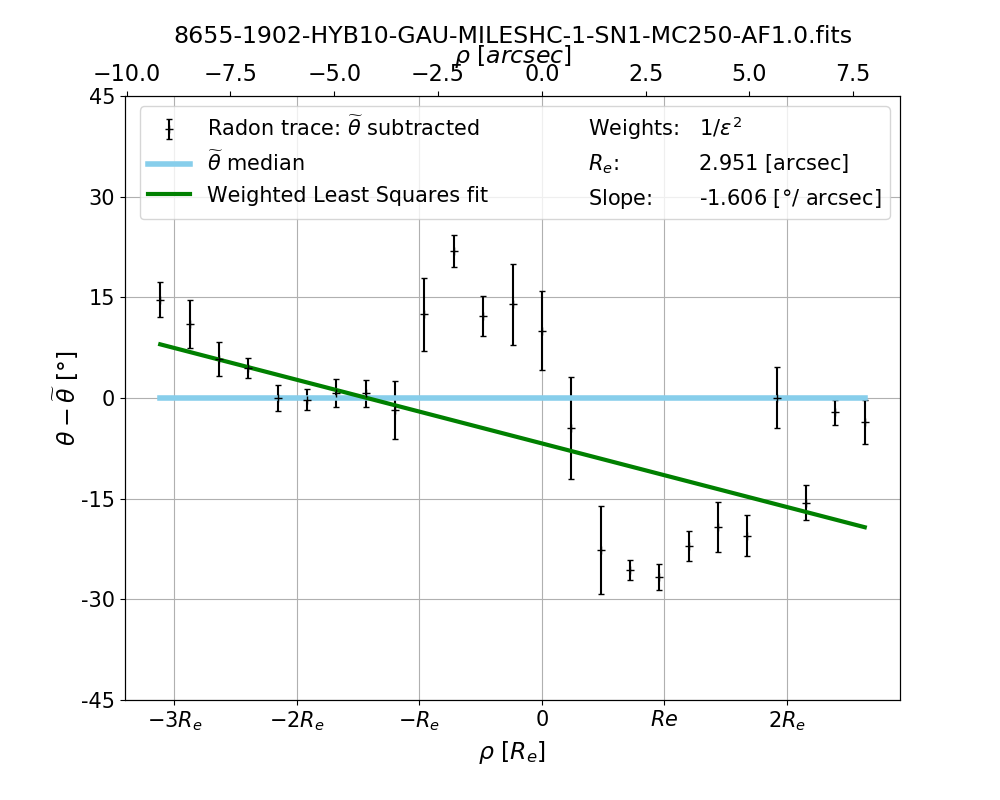
\includegraphics[width=0.31\textwidth]{Images/WLSFITS/CPSB/8655-1902.png}
    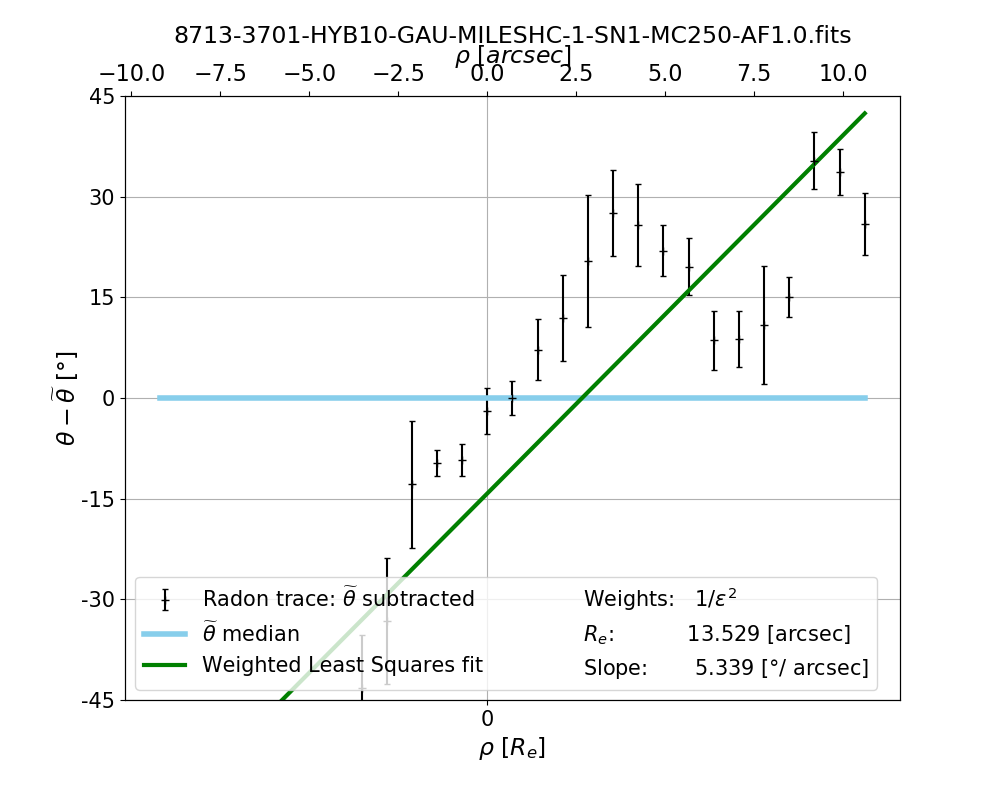
\includegraphics[width=0.31\textwidth]{Images/WLSFITS/CPSB/8713-3701.png}
    % 
%
    \caption{Radon transform trace profiles of stellar velocity maps of the main sample CPSBs (set 1 of 2). The RT input parameters are: $SNCUT=1$ and $MC\_ITER=250$. The RT trace profiles have been subtracted from the median value $\widetilde\theta$ (plotted in light blue) and superimposed with a weighted least squares linear fit of the trace slope (plotted in green). Calculated values of the slope and some salient parameters are displayed in the legend.}
    \label{fig:Radon-traces-CPSB-WLSFITS-1}
\end{figure*}

\begin{figure*}
    \centering
    %
    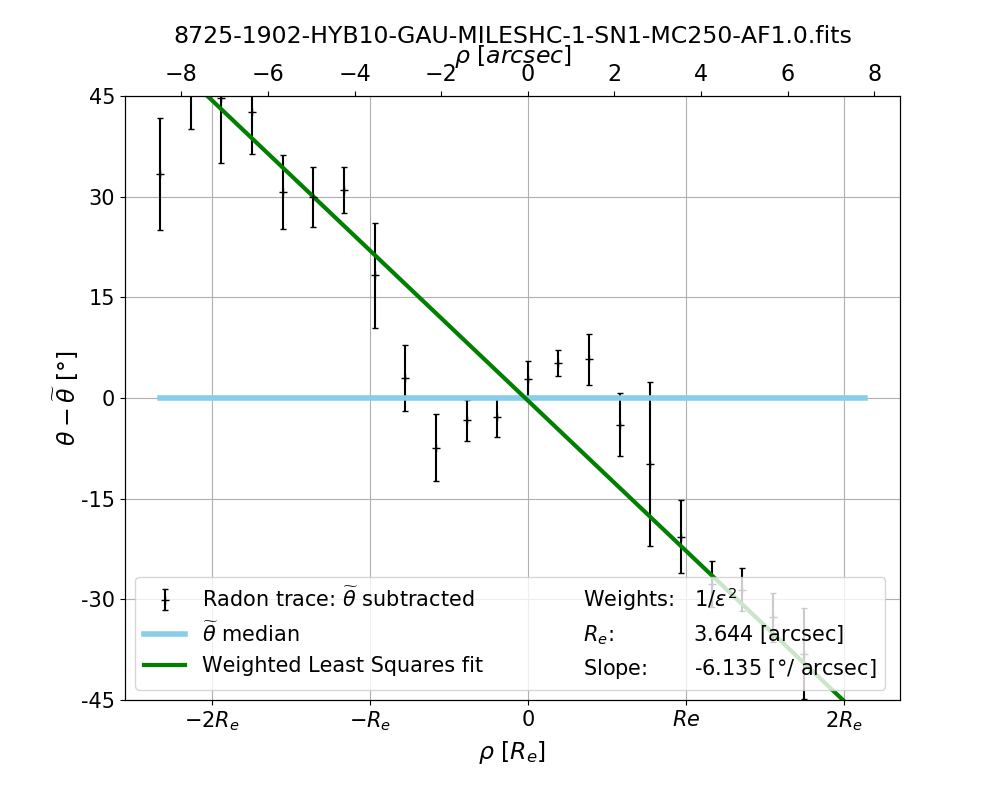
\includegraphics[width=0.31\textwidth]{Images/WLSFITS/CPSB/8725-1902.png}
    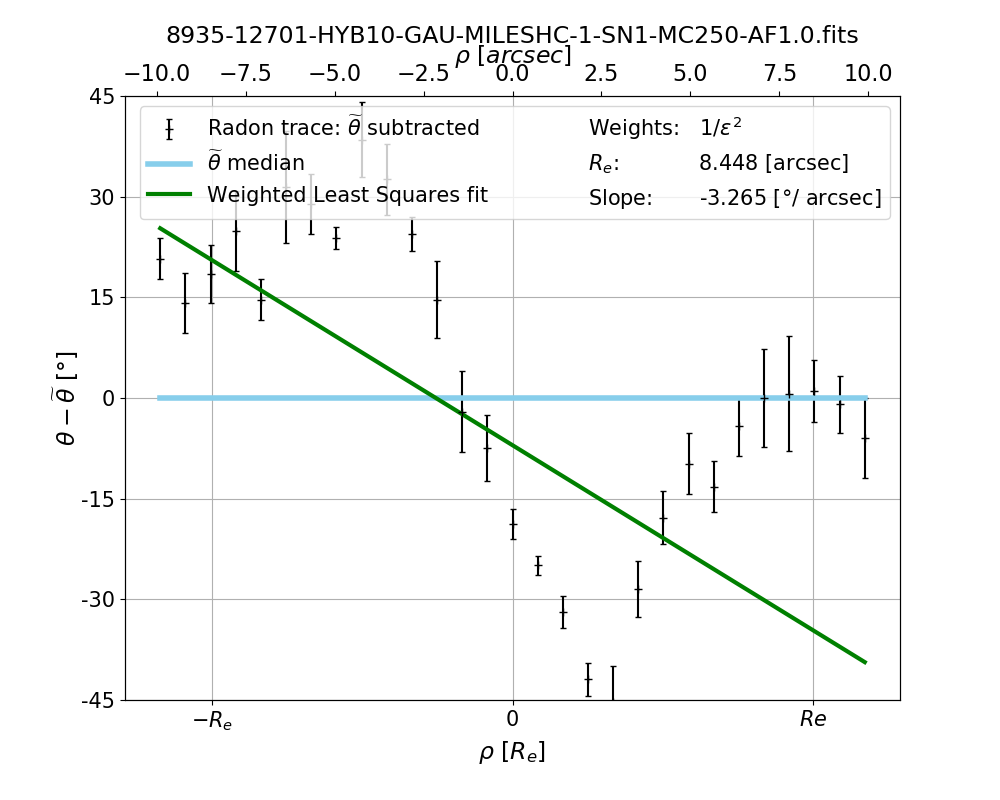
\includegraphics[width=0.31\textwidth]{Images/WLSFITS/CPSB/8935-12701.png}
    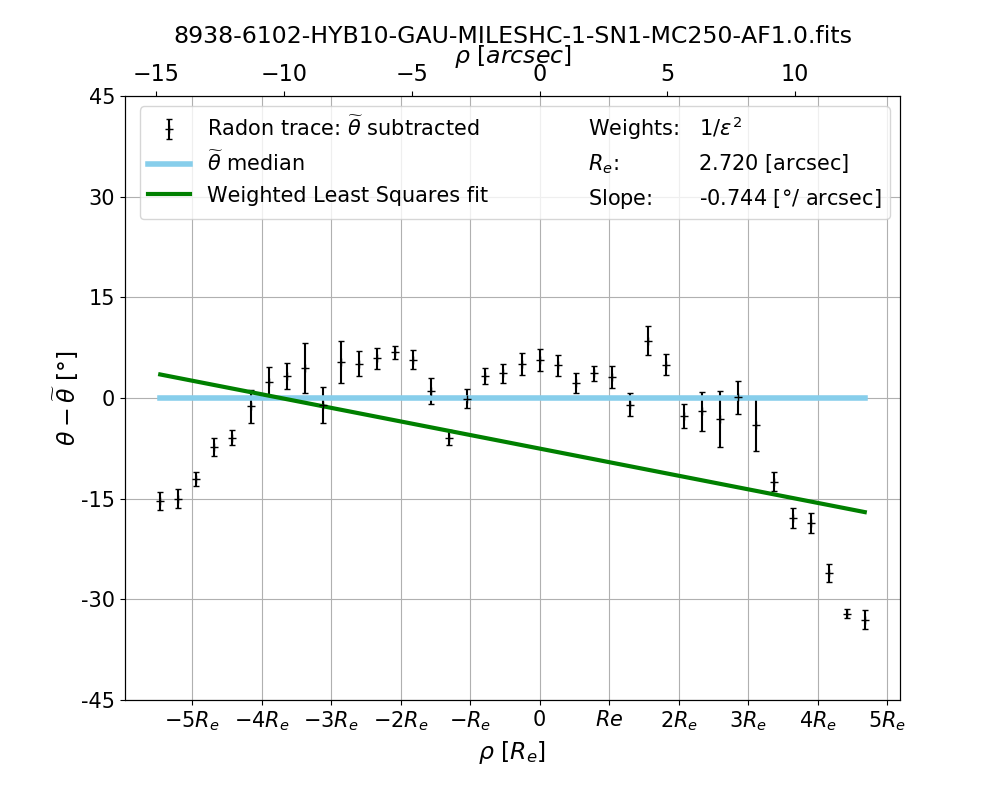
\includegraphics[width=0.31\textwidth]{Images/WLSFITS/CPSB/8938-6102.png}
    %
    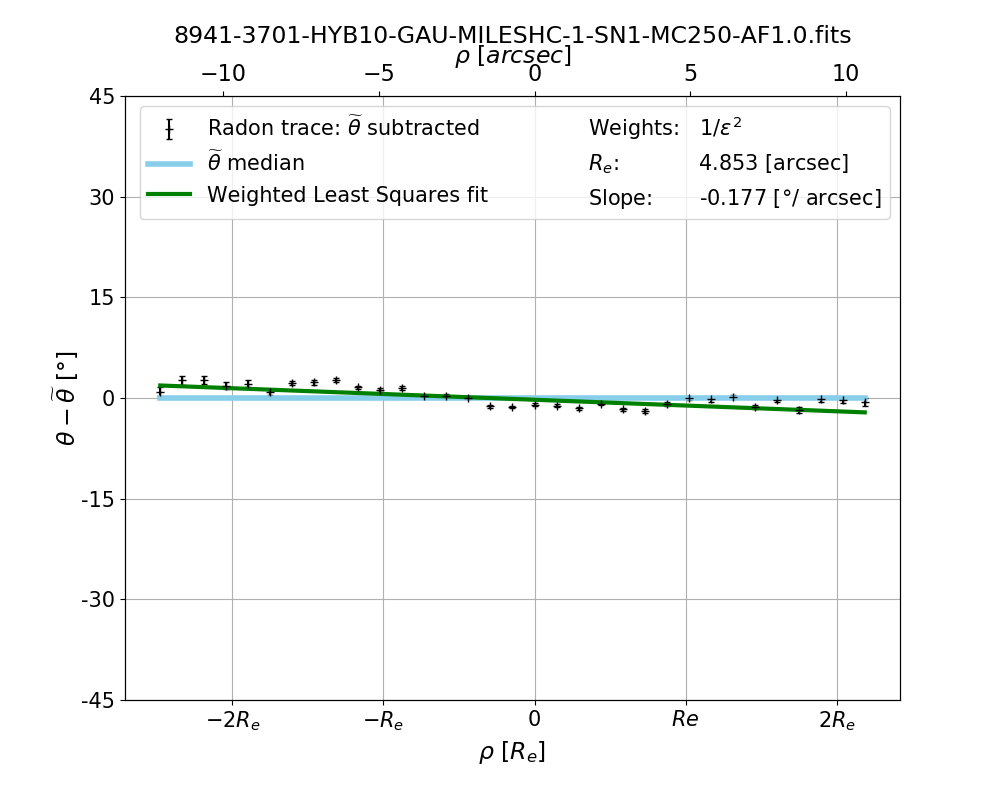
\includegraphics[width=0.31\textwidth]{Images/WLSFITS/CPSB/8941-3701.png}
    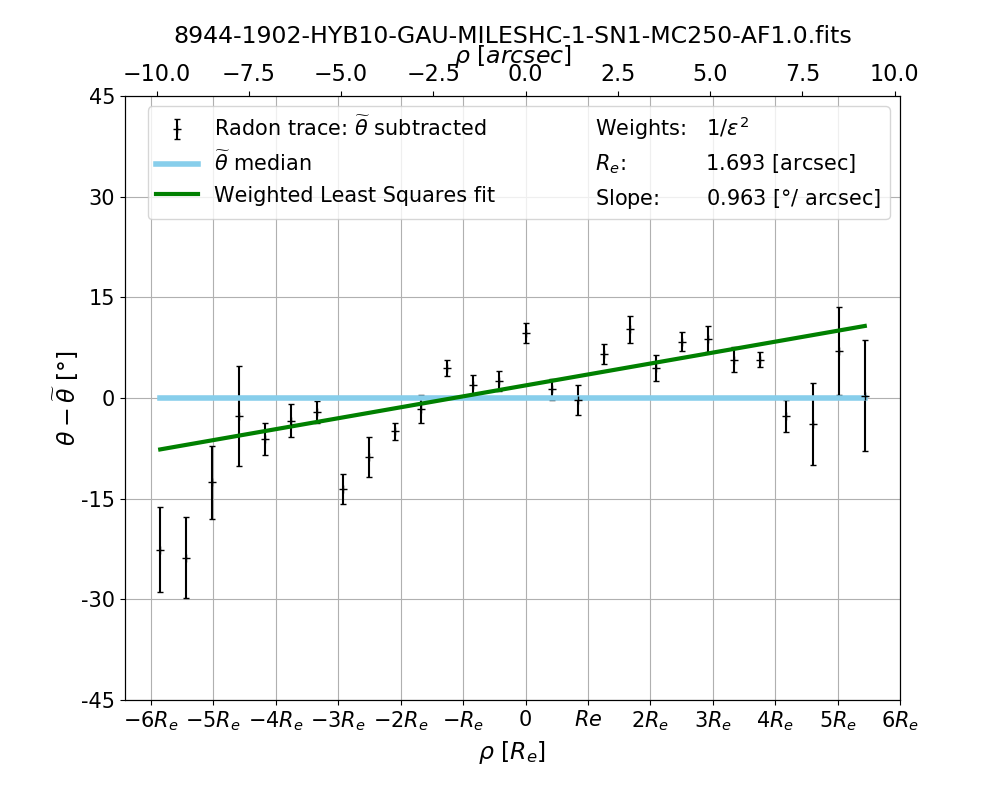
\includegraphics[width=0.31\textwidth]{Images/WLSFITS/CPSB/8944-1902.png}
    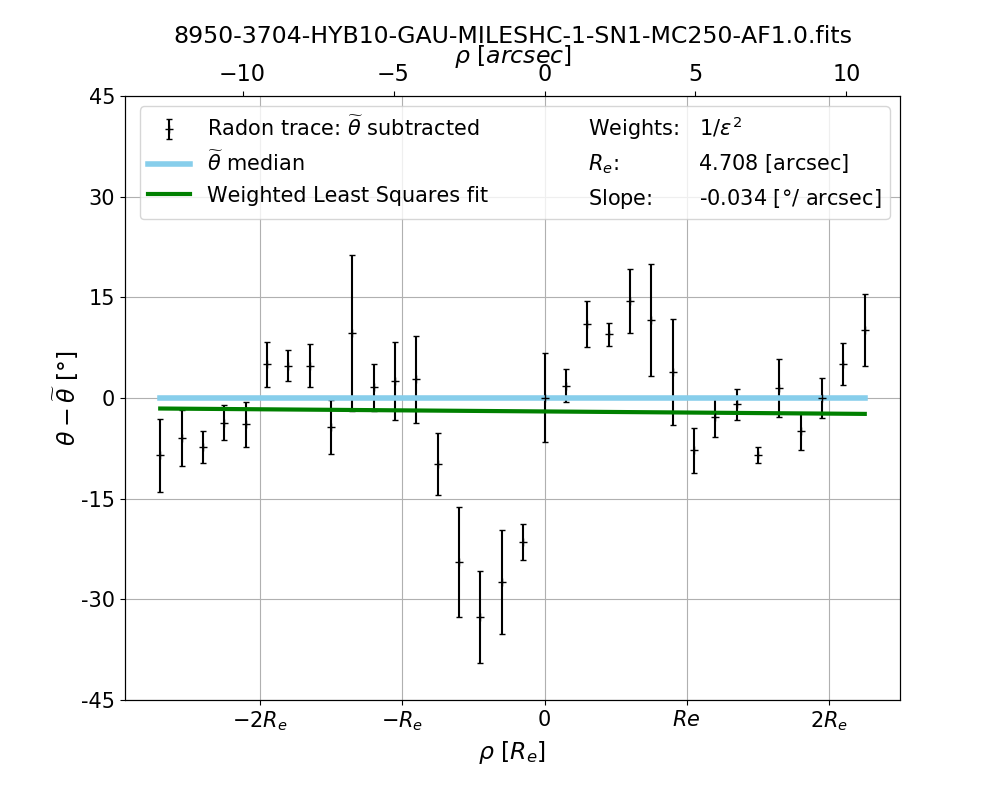
\includegraphics[width=0.31\textwidth]{Images/WLSFITS/CPSB/8950-3704.png}
    %
    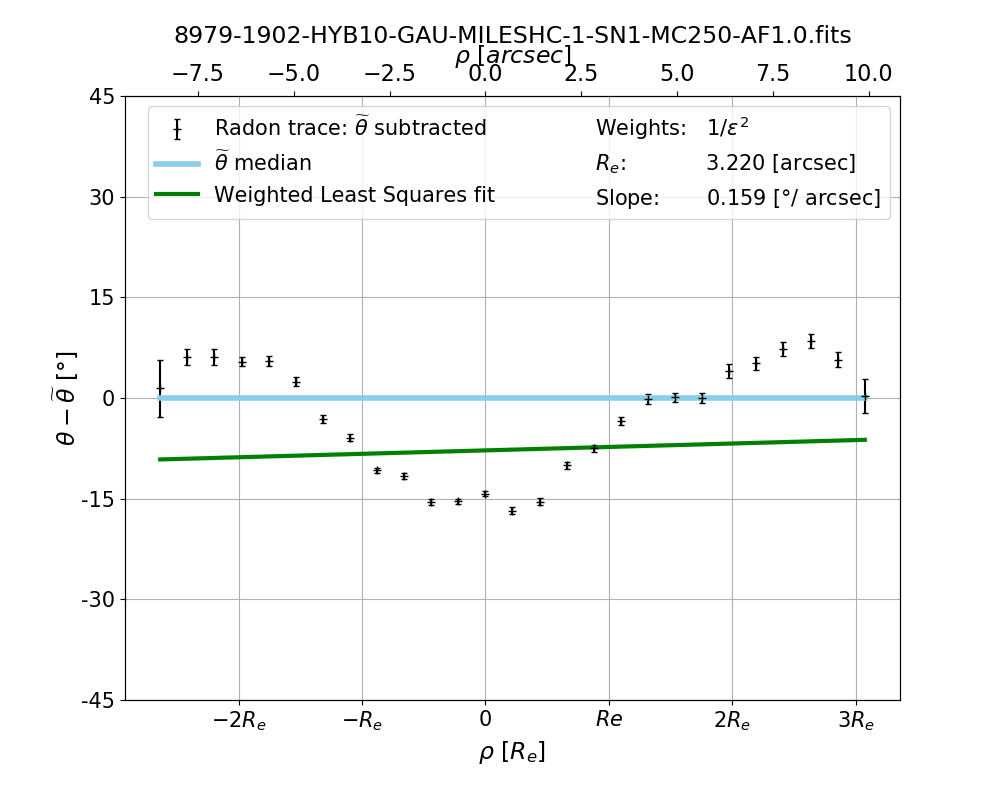
\includegraphics[width=0.31\textwidth]{Images/WLSFITS/CPSB/8979-1902.png}
    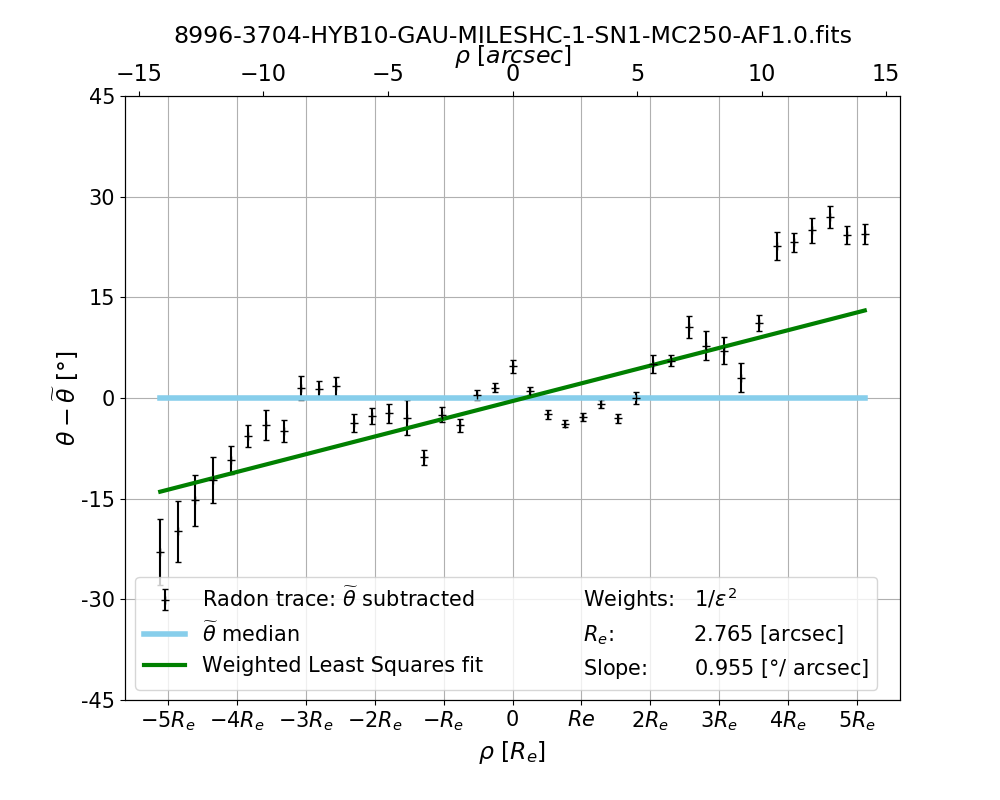
\includegraphics[width=0.31\textwidth]{Images/WLSFITS/CPSB/8996-3704.png}
    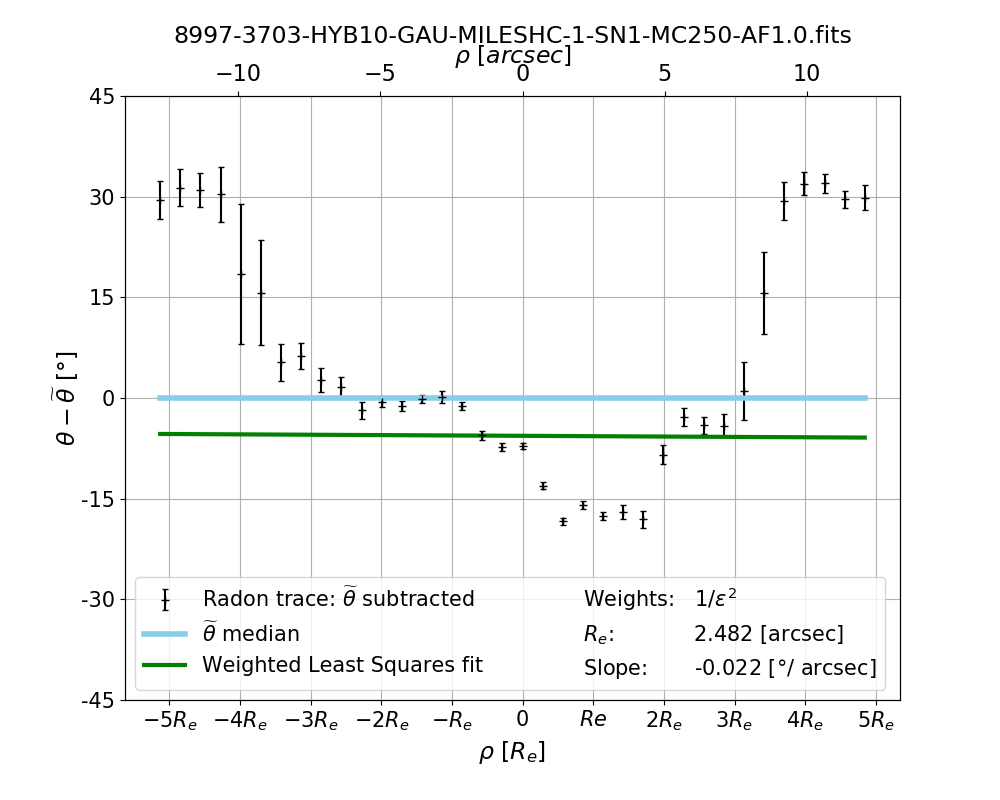
\includegraphics[width=0.31\textwidth]{Images/WLSFITS/CPSB/8997-3703.png}
    %
    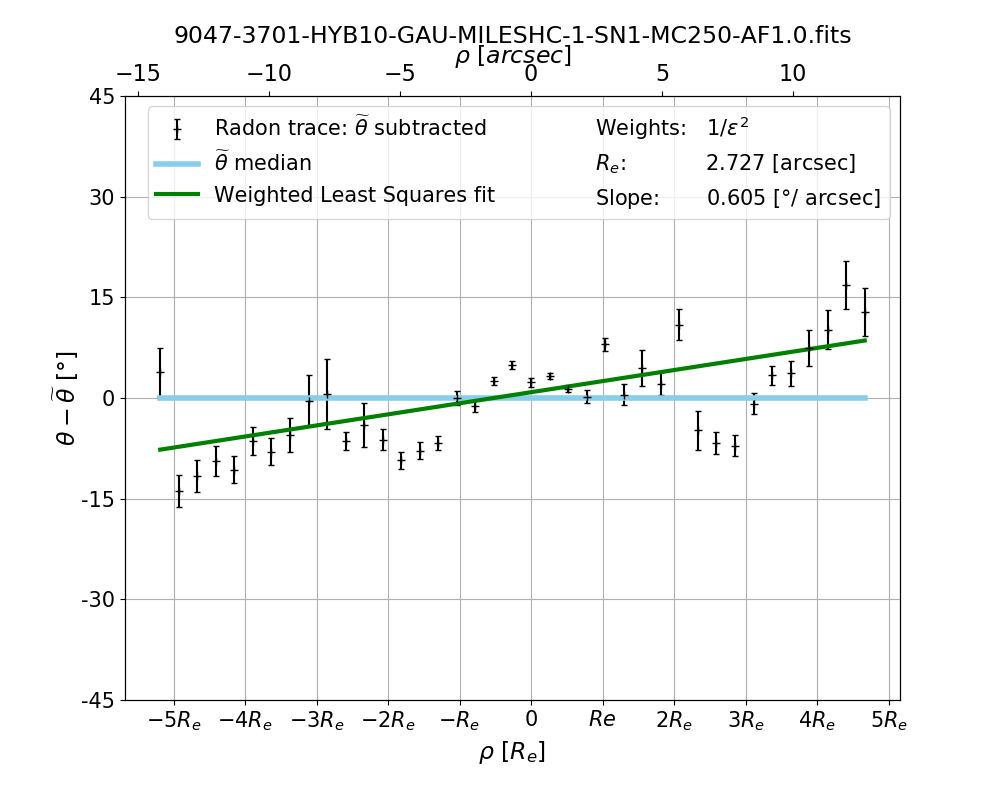
\includegraphics[width=0.31\textwidth]{Images/WLSFITS/CPSB/9047-3701.png}
    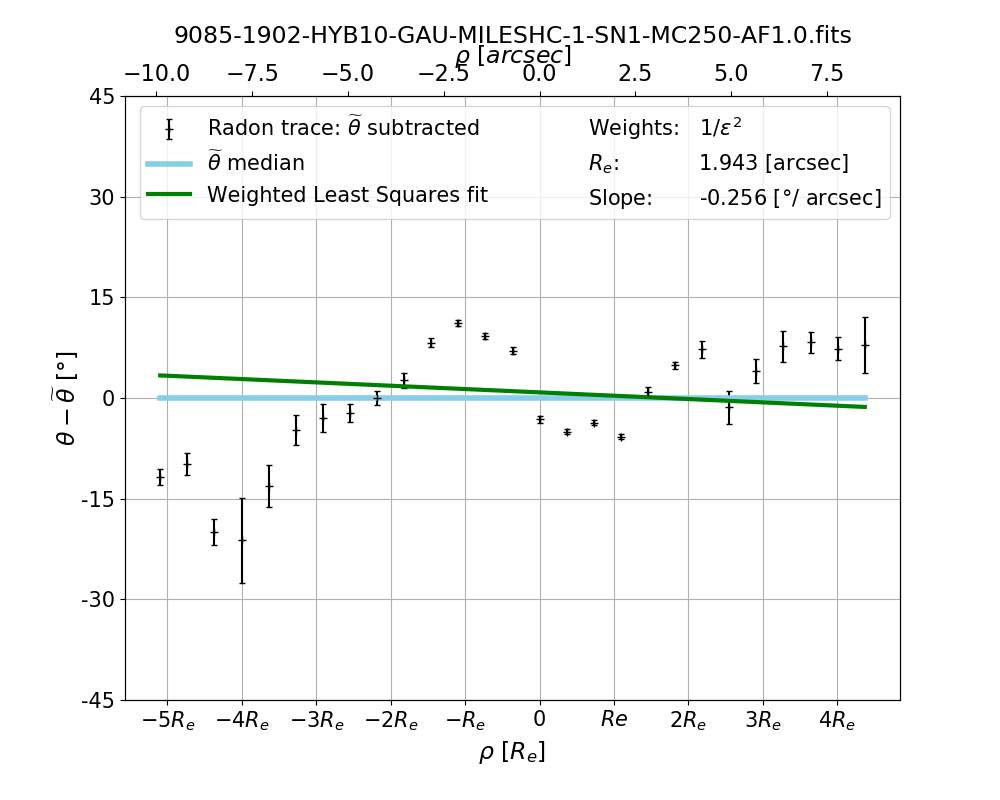
\includegraphics[width=0.31\textwidth]{Images/WLSFITS/CPSB/9085-1902.png}
    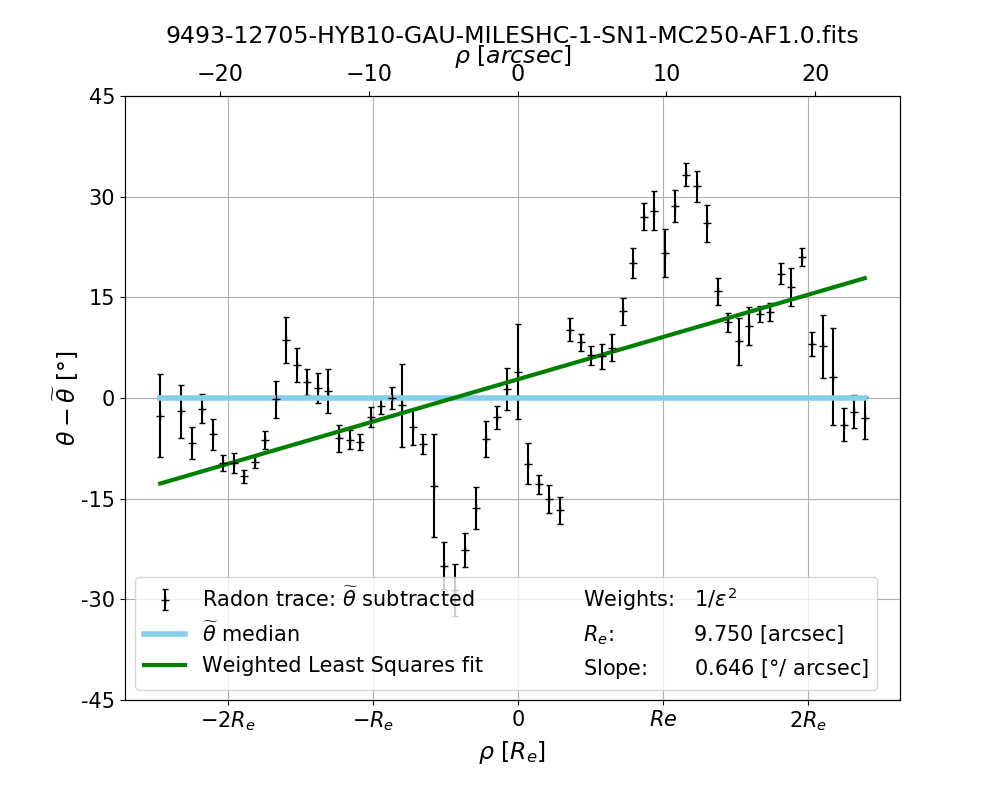
\includegraphics[width=0.31\textwidth]{Images/WLSFITS/CPSB/9493-12705.png}
    %
    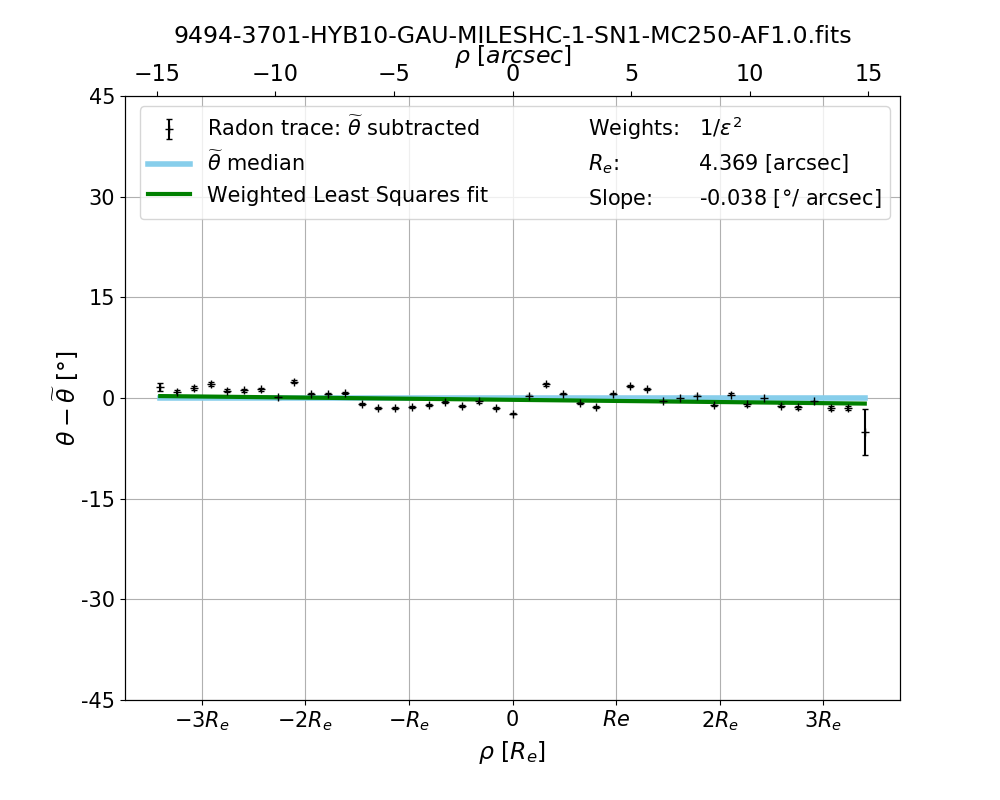
\includegraphics[width=0.31\textwidth]{Images/WLSFITS/CPSB/9494-3701.png}
    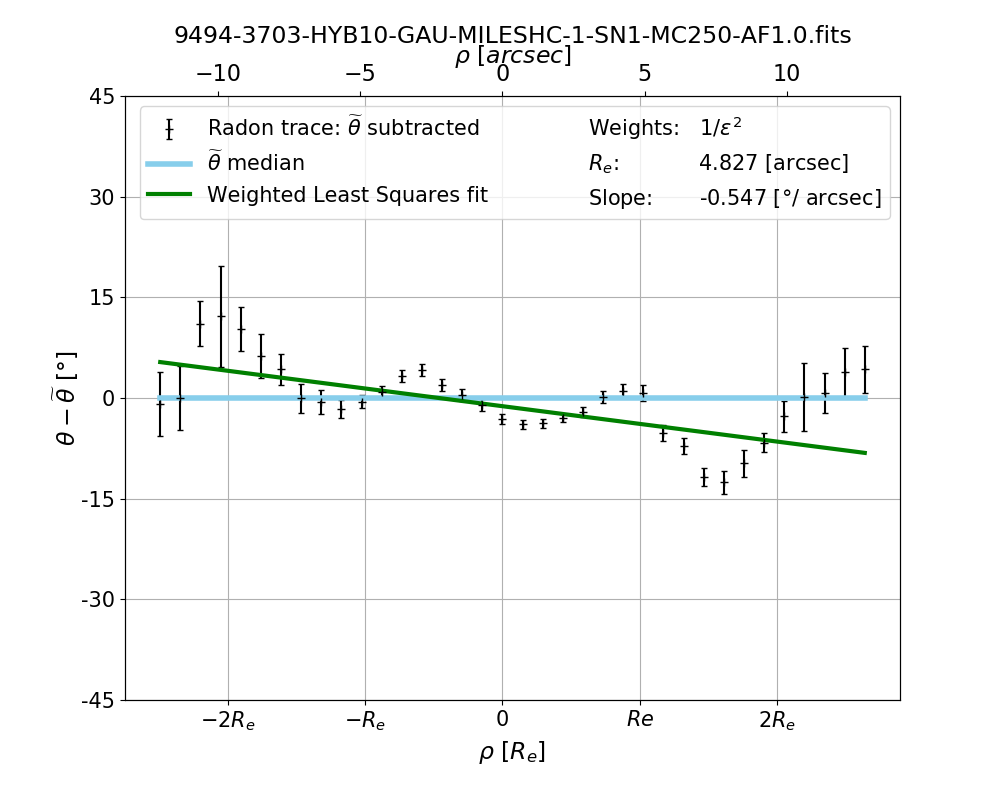
\includegraphics[width=0.31\textwidth]{Images/WLSFITS/CPSB/9494-3703.png}
    %
%
    \caption{Radon transform trace plots of the main sample CPSBs (set 2 0f 2). The content description is as per Figure \ref{fig:Radon-traces-CPSB-WLSFITS-1}.}
    \label{fig:Radon-traces-CPSB-WLSFITS-2}
\end{figure*}

% CC0s ================================

\begin{figure*}
    \centering
    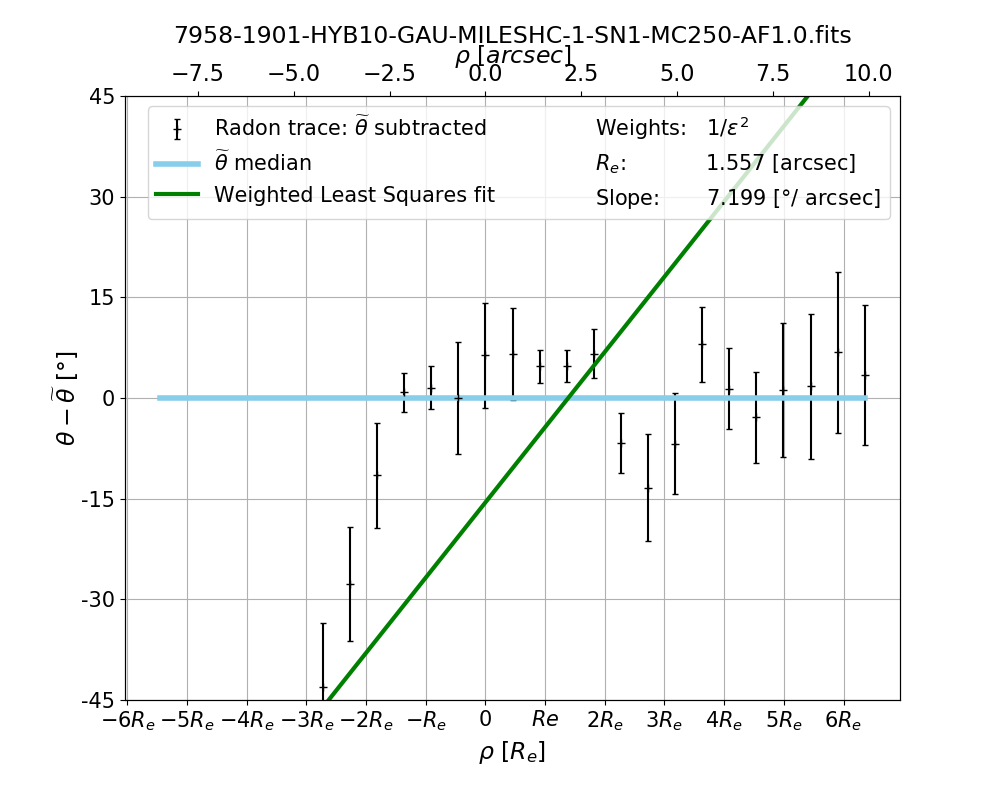
\includegraphics[width=0.31\textwidth]{Images/WLSFITS/CC0/7958-1901.png}
    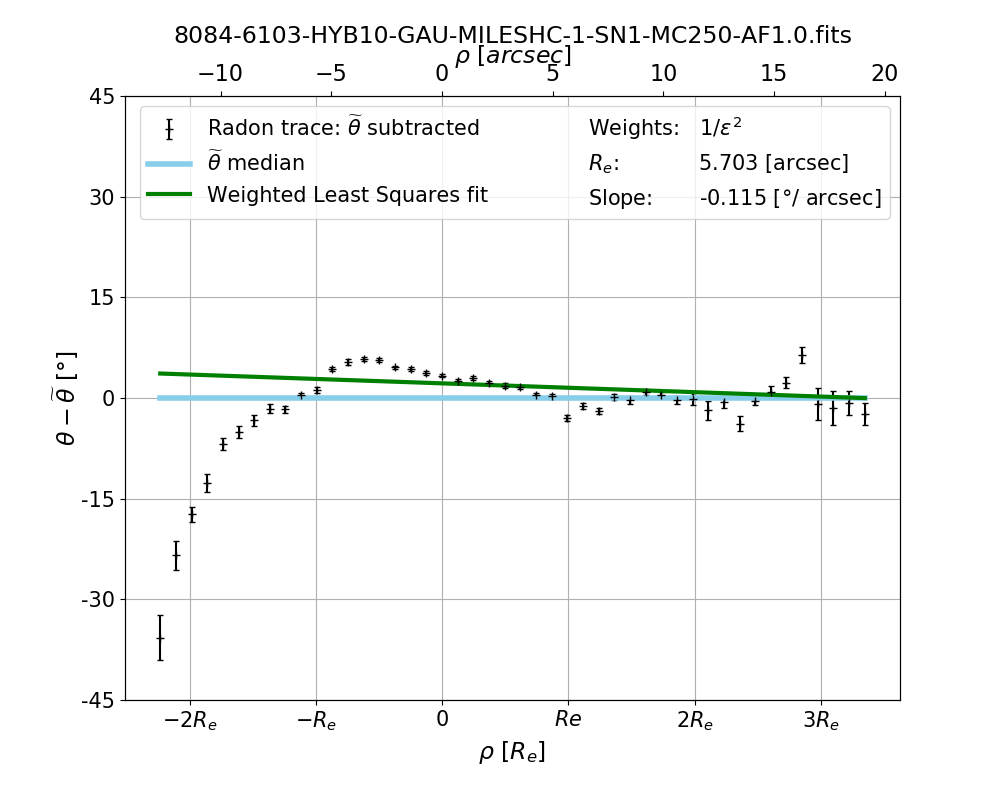
\includegraphics[width=0.31\textwidth]{Images/WLSFITS/CC0/8084-6103.png}
    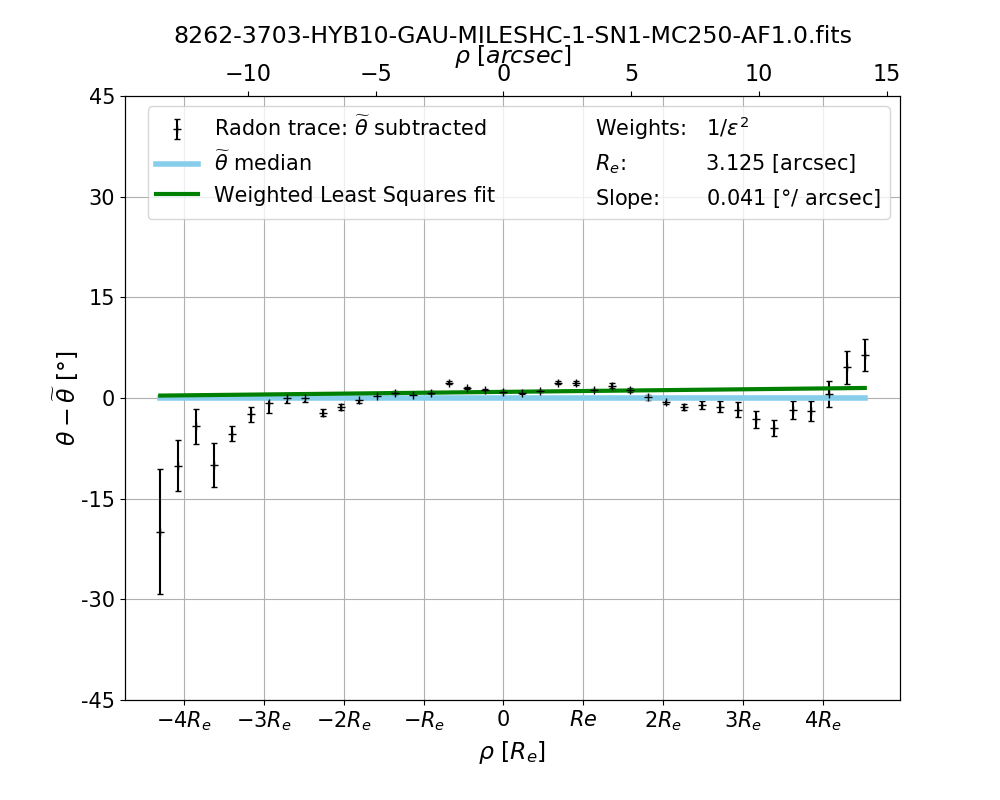
\includegraphics[width=0.31\textwidth]{Images/WLSFITS/CC0/8262-3703.png}
    %
    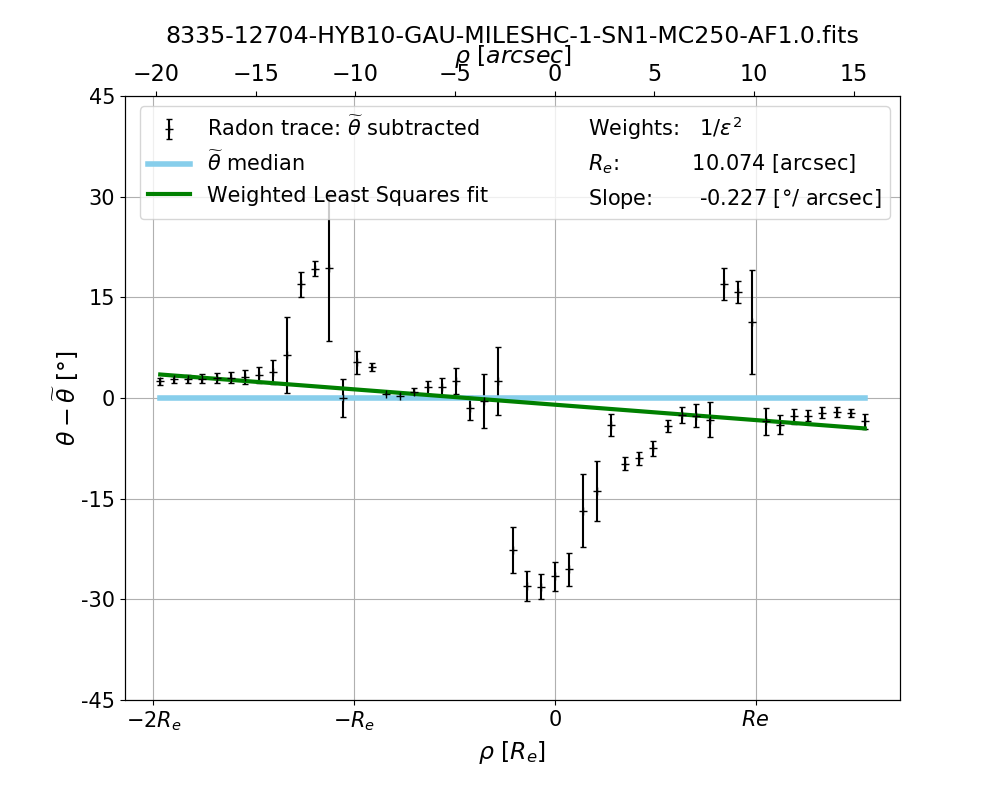
\includegraphics[width=0.31\textwidth]{Images/WLSFITS/CC0/8335-12704.png}
    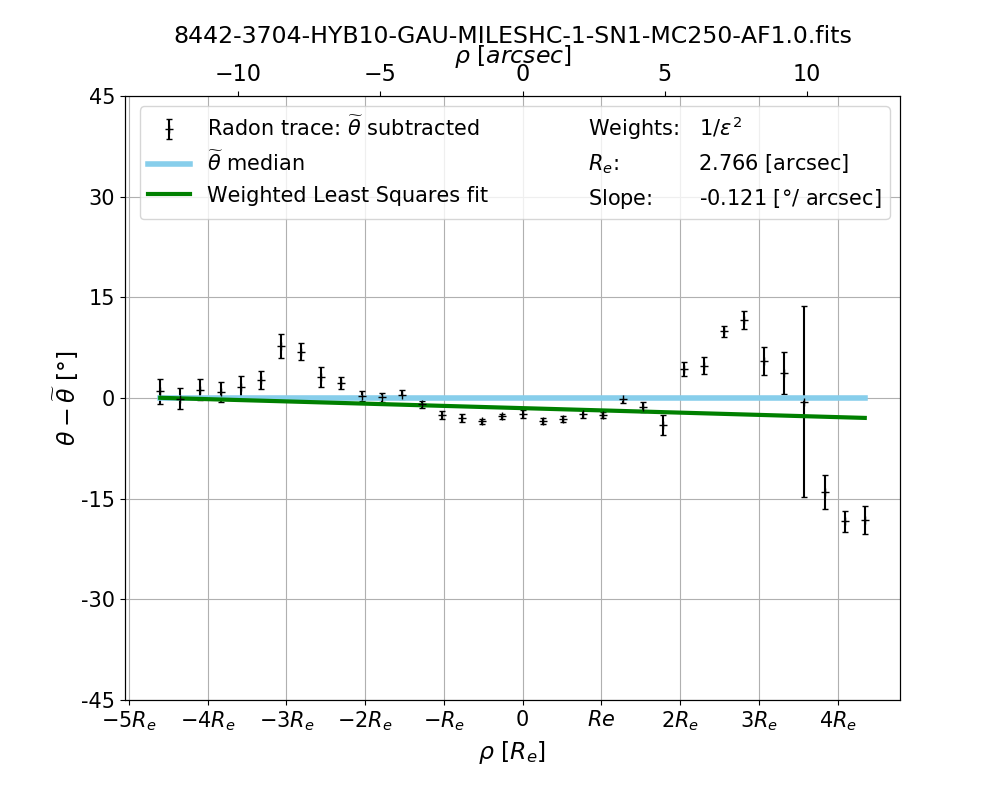
\includegraphics[width=0.31\textwidth]{Images/WLSFITS/CC0/8442-3704.png}
    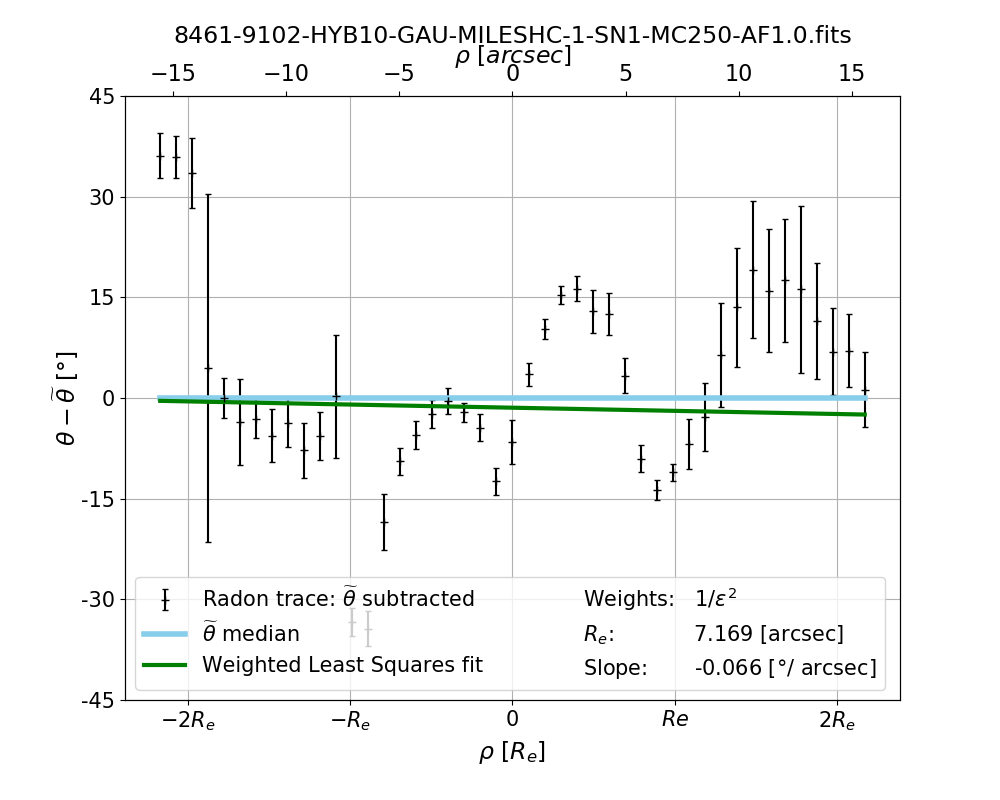
\includegraphics[width=0.31\textwidth]{Images/WLSFITS/CC0/8461-9102.png}
    %
    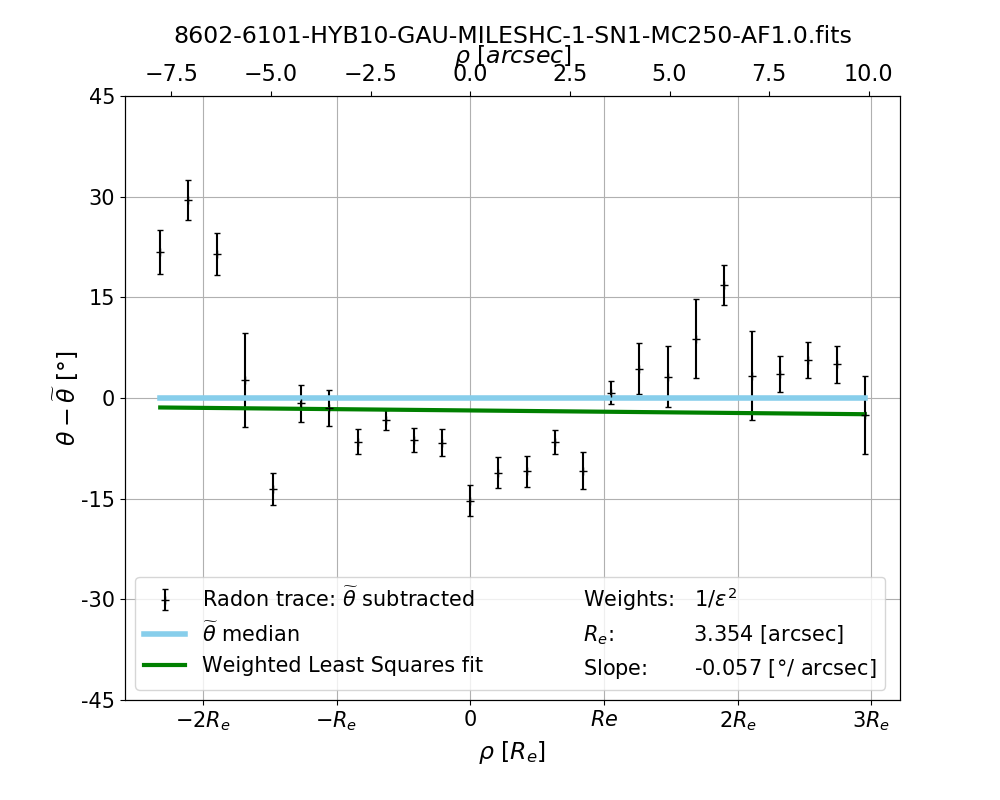
\includegraphics[width=0.31\textwidth]{Images/WLSFITS/CC0/8602-6101.png}
    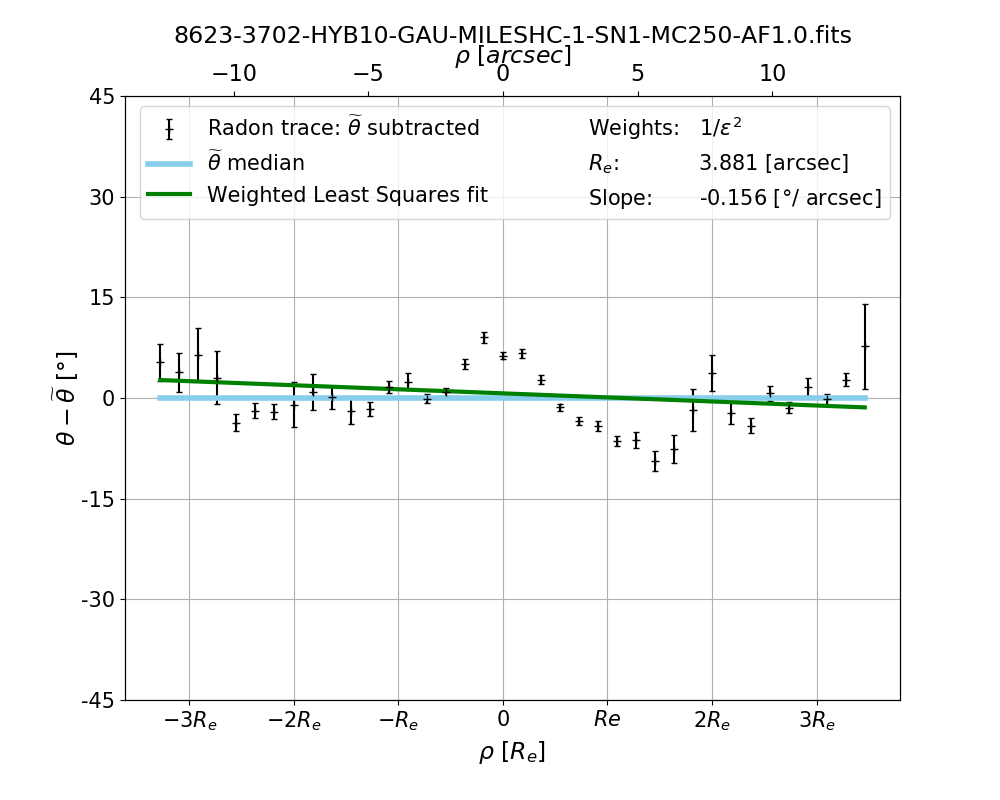
\includegraphics[width=0.31\textwidth]{Images/WLSFITS/CC0/8623-3702.png}
    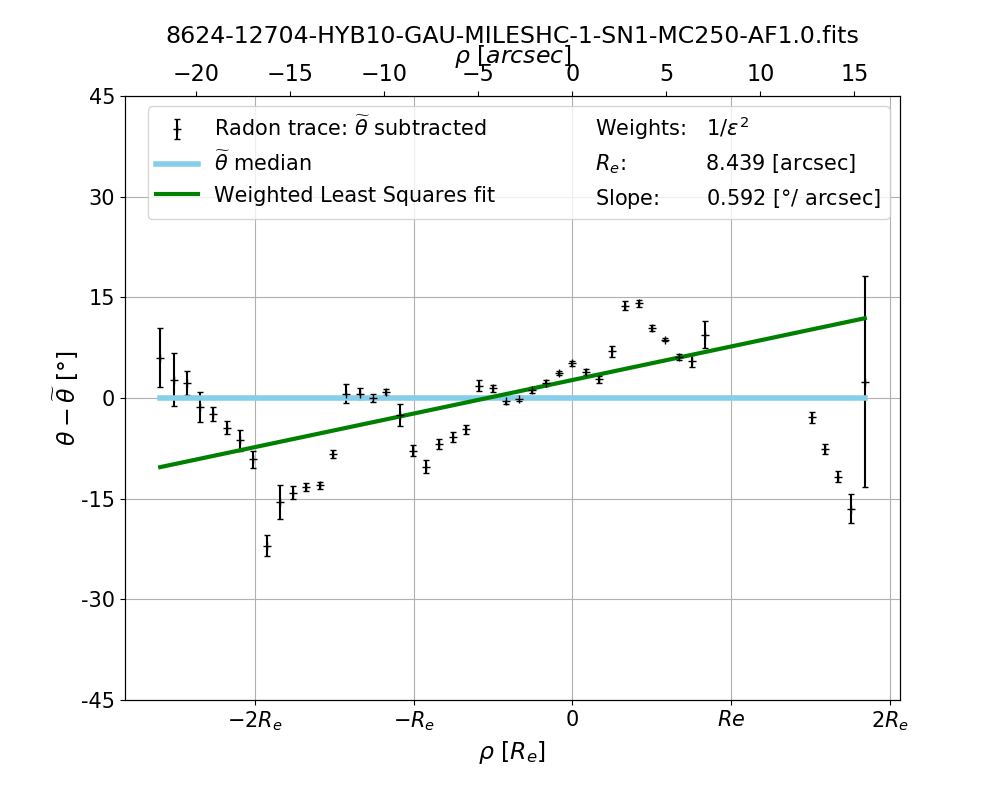
\includegraphics[width=0.31\textwidth]{Images/WLSFITS/CC0/8624-12704.png}
    %
    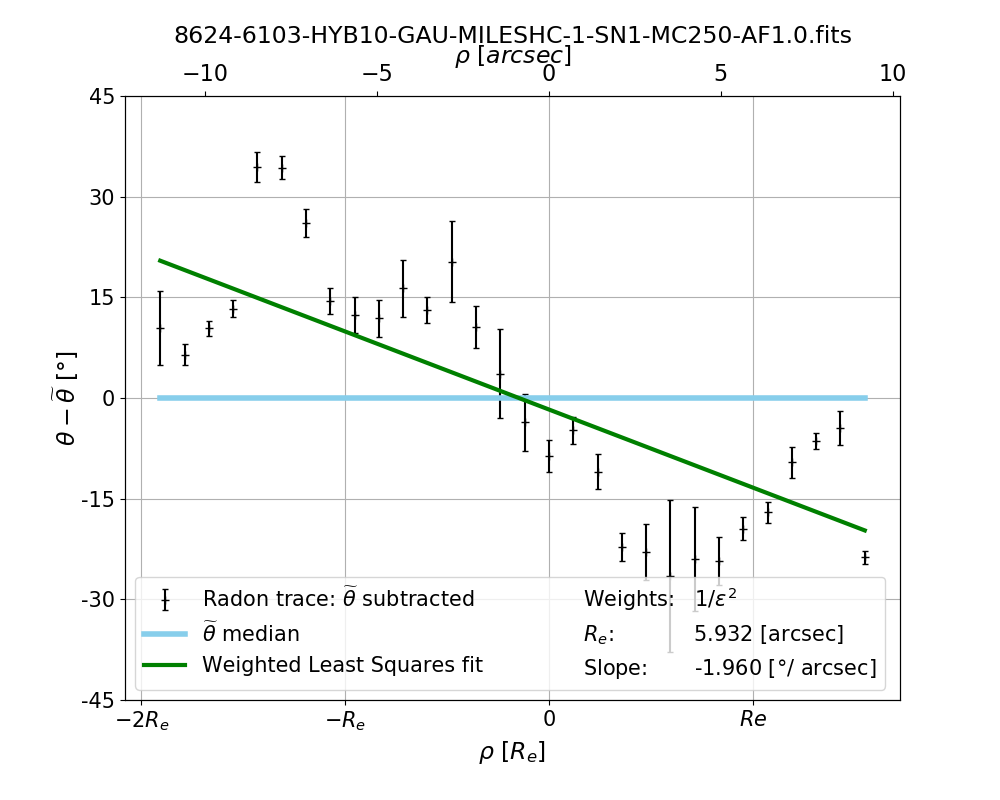
\includegraphics[width=0.31\textwidth]{Images/WLSFITS/CC0/8624-6103.png}
    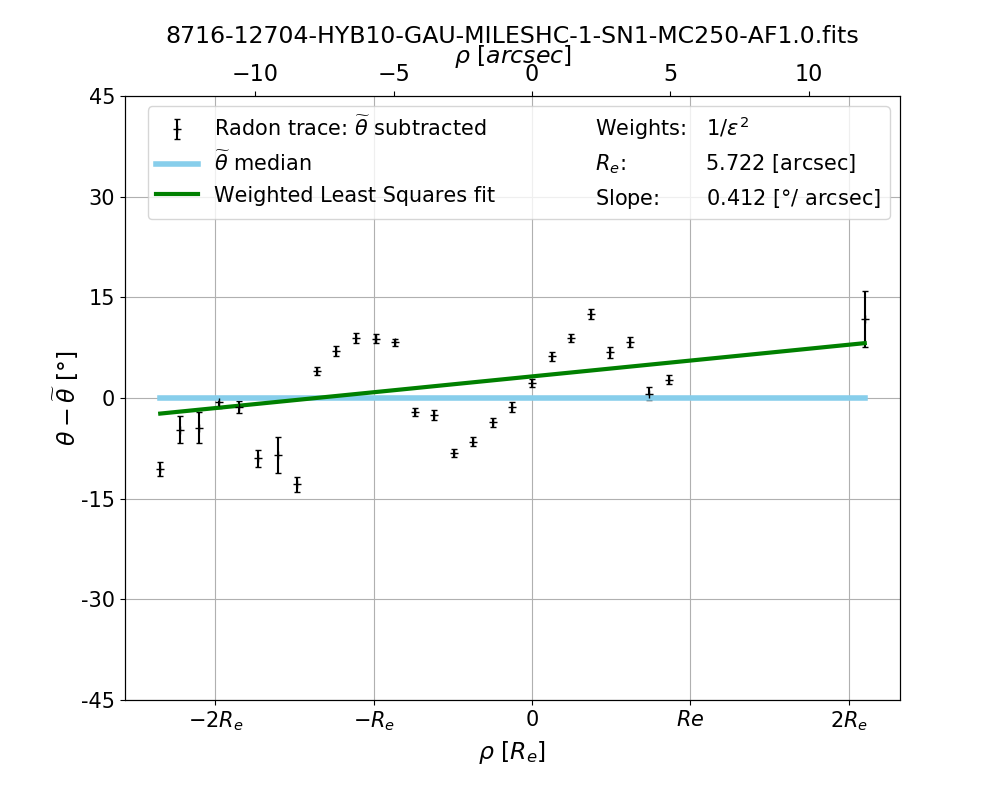
\includegraphics[width=0.31\textwidth]{Images/WLSFITS/CC0/8716-12704.png}
    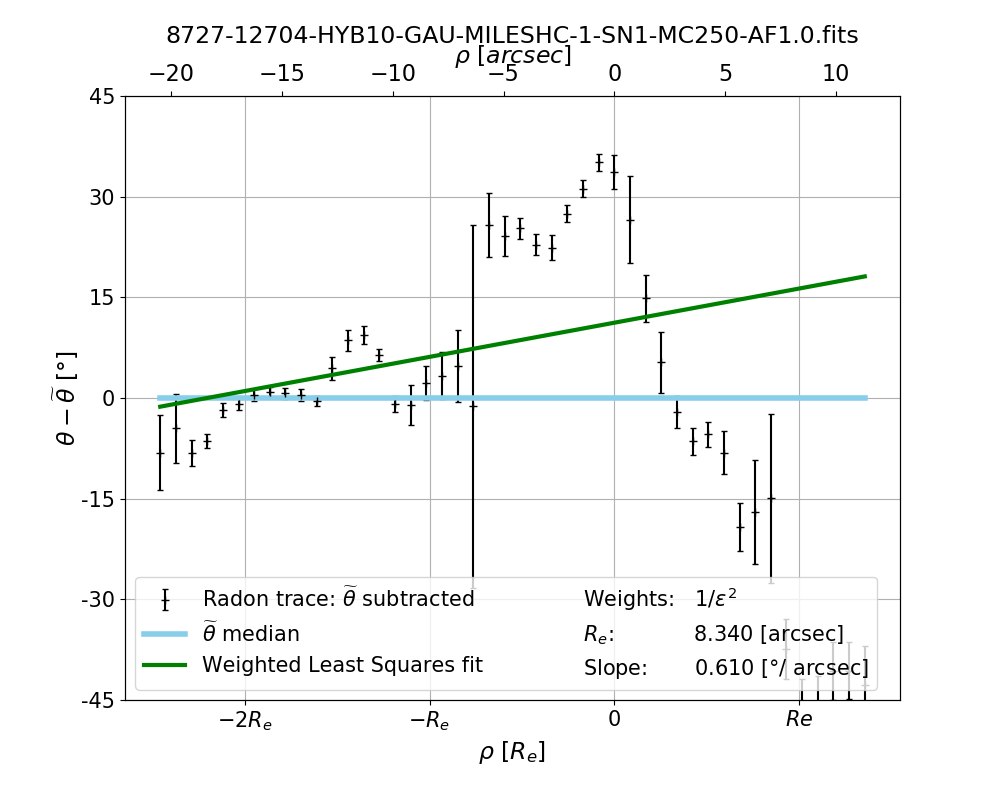
\includegraphics[width=0.31\textwidth]{Images/WLSFITS/CC0/8727-12704.png}
    %
    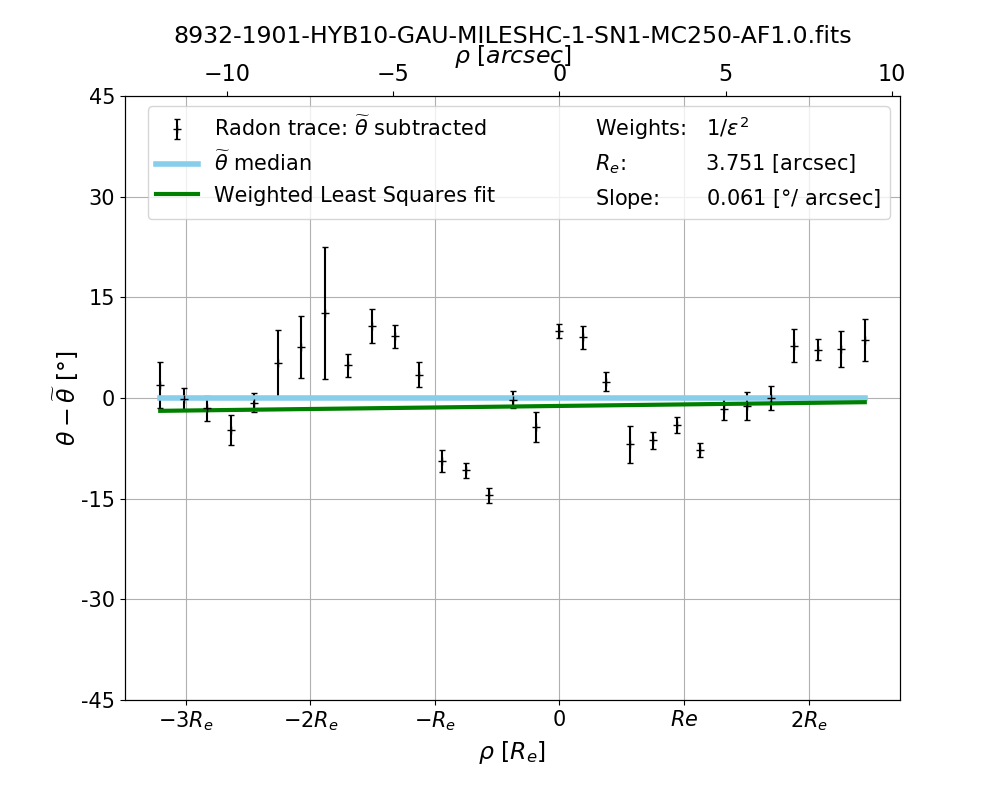
\includegraphics[width=0.31\textwidth]{Images/WLSFITS/CC0/8932-1901.png}
    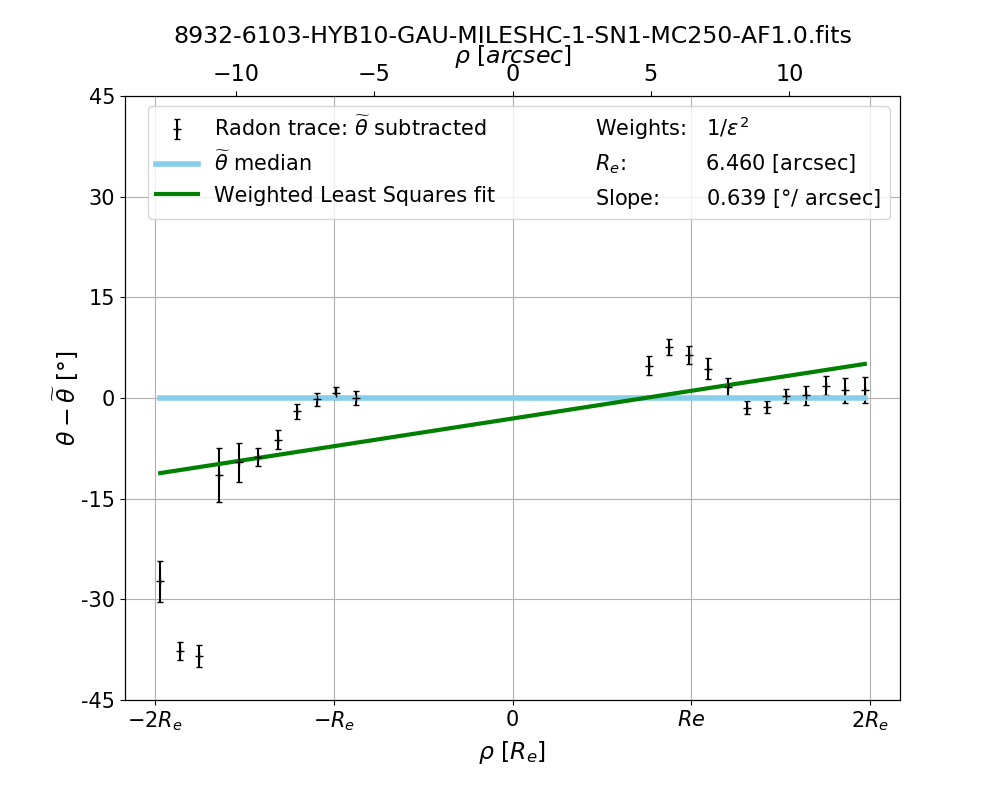
\includegraphics[width=0.31\textwidth]{Images/WLSFITS/CC0/8932-6103.png}
    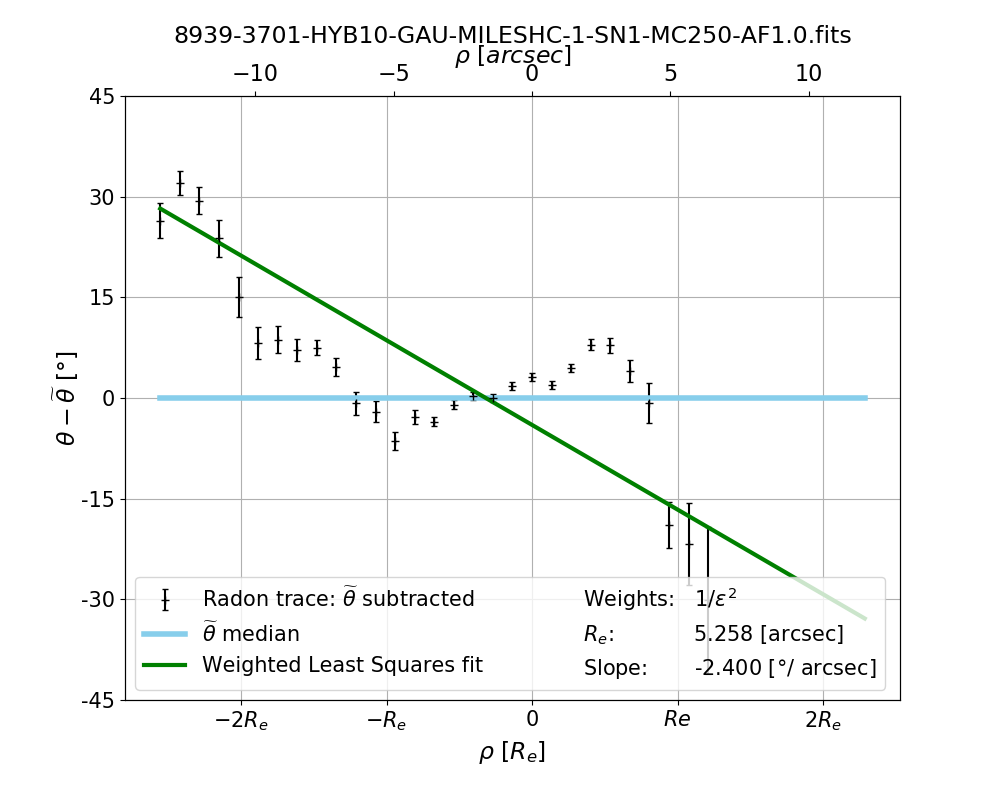
\includegraphics[width=0.31\textwidth]{Images/WLSFITS/CC0/8939-3701.png}
%
    \caption{Radon transform trace plots of the control galaxy sample CC0 (set 1 0f 2). The content description is as per Figure \ref{fig:Radon-traces-CPSB-WLSFITS-1}.}
    \label{fig:Radon-traces-CC0-WLSFITS-1}
\end{figure*}

\begin{figure*}
    \centering
    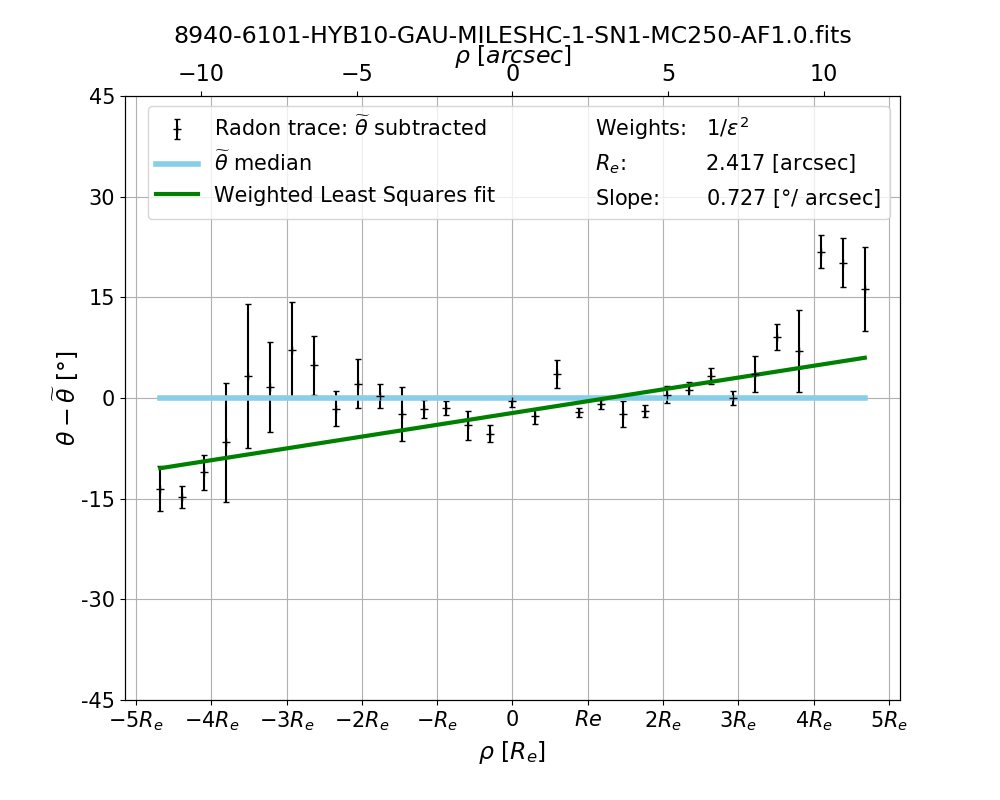
\includegraphics[width=0.31\textwidth]{Images/WLSFITS/CC0/8940-6101.png}
    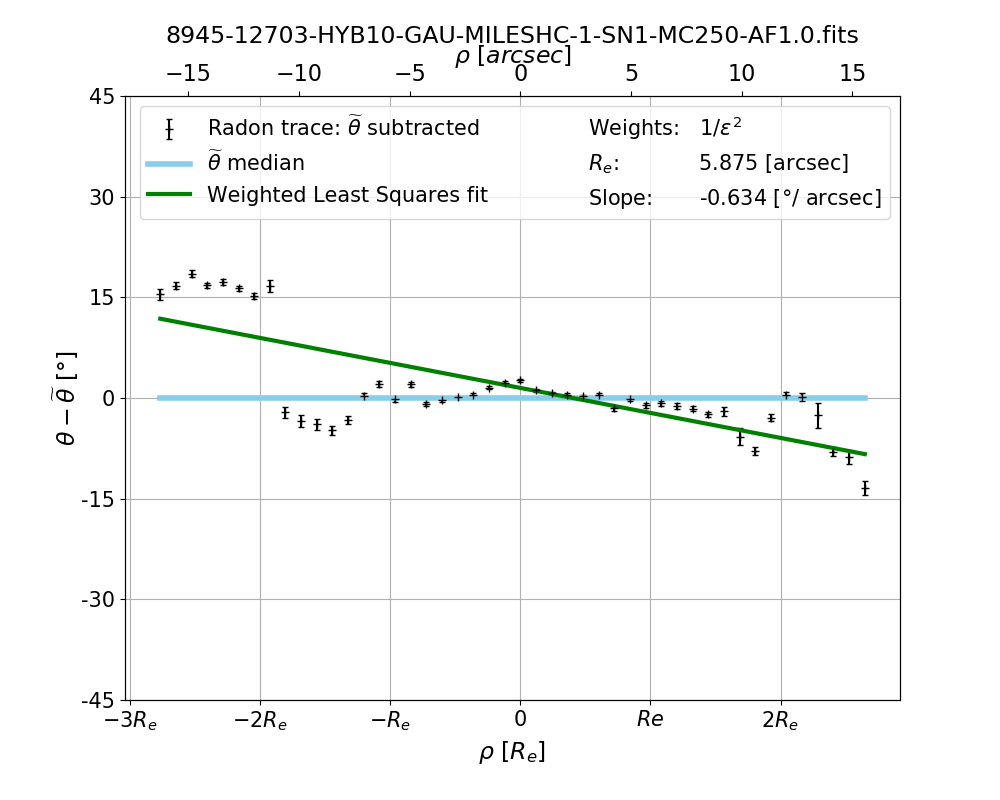
\includegraphics[width=0.31\textwidth]{Images/WLSFITS/CC0/8945-12703.png}
    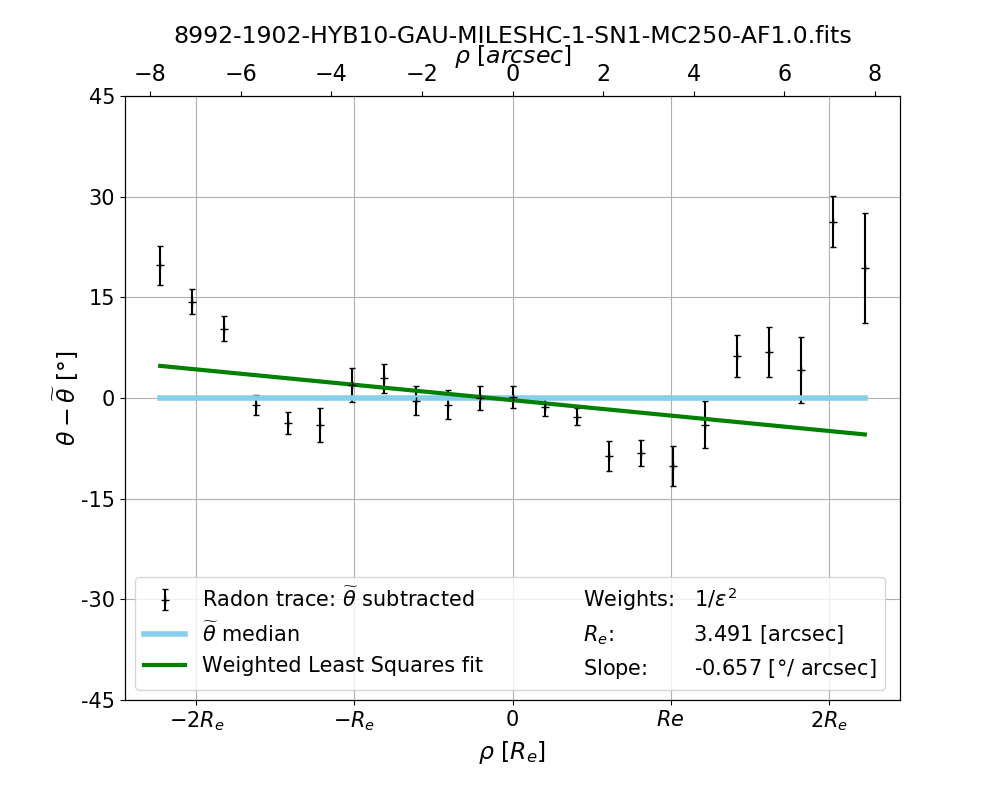
\includegraphics[width=0.31\textwidth]{Images/WLSFITS/CC0/8992-1902.png}
    %
    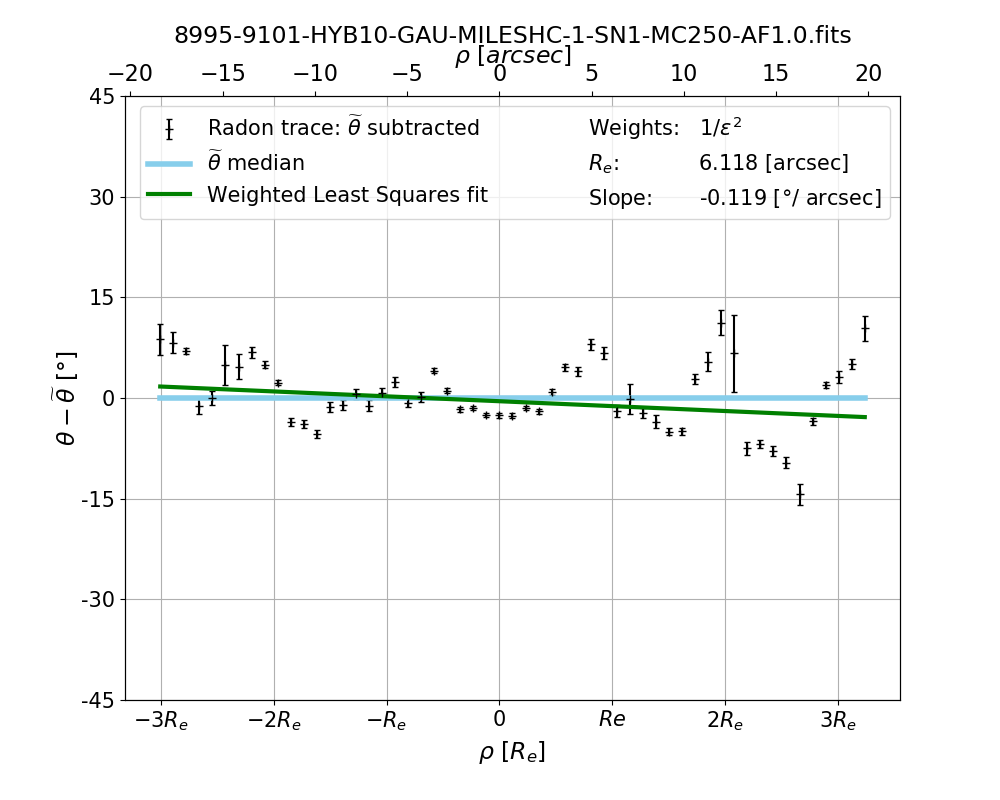
\includegraphics[width=0.31\textwidth]{Images/WLSFITS/CC0/8995-9101.png}
    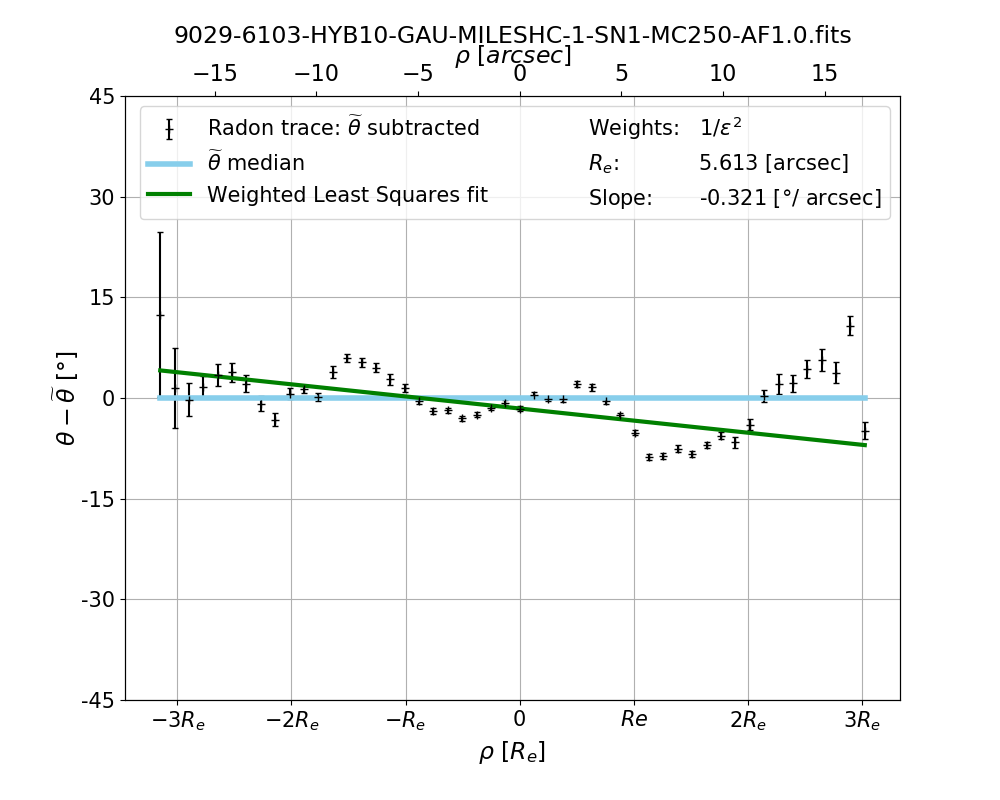
\includegraphics[width=0.31\textwidth]{Images/WLSFITS/CC0/9029-6103.png}
    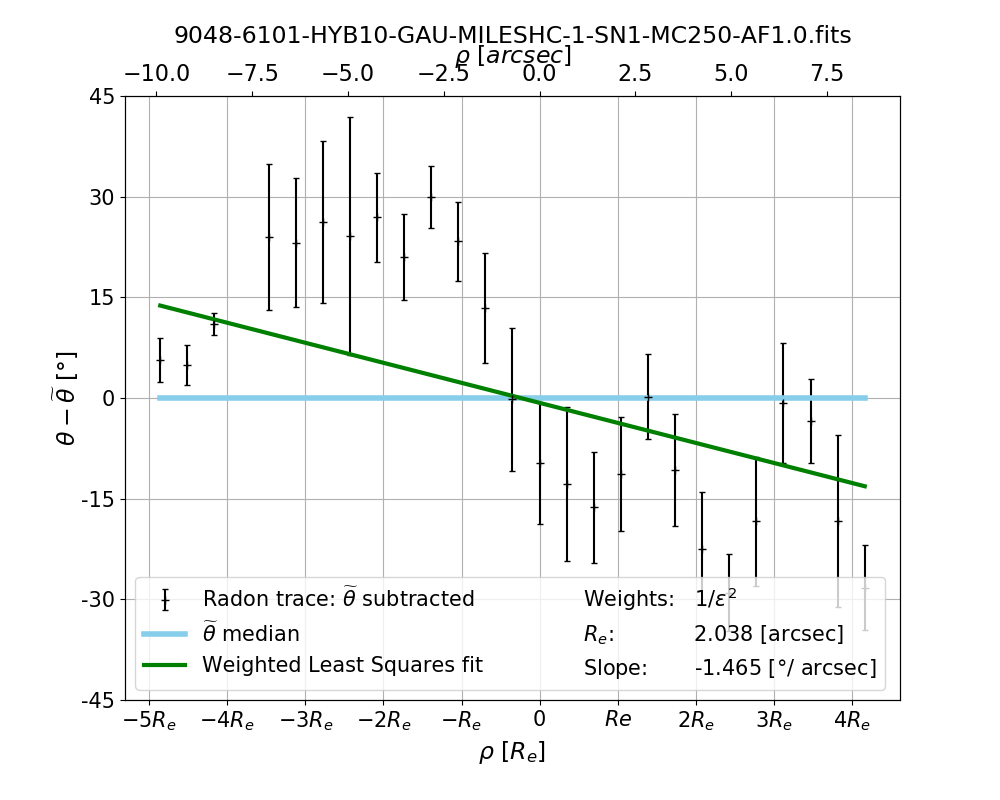
\includegraphics[width=0.31\textwidth]{Images/WLSFITS/CC0/9048-6101.png}
    % 
    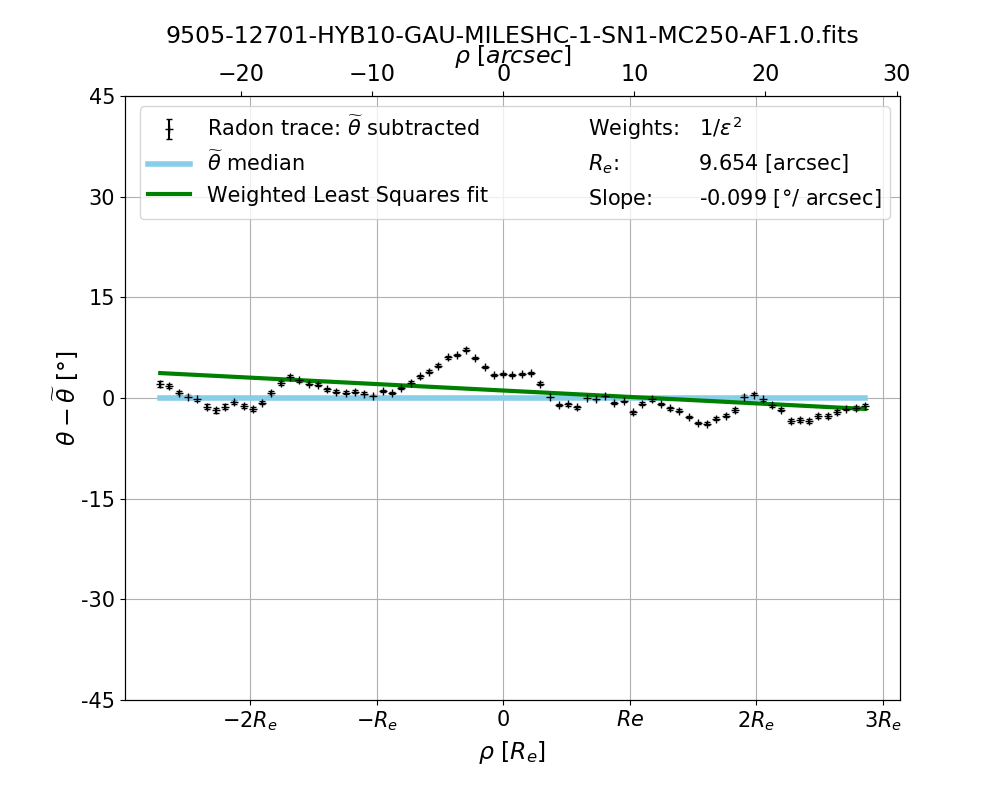
\includegraphics[width=0.31\textwidth]{Images/WLSFITS/CC0/9505-12701.png}
    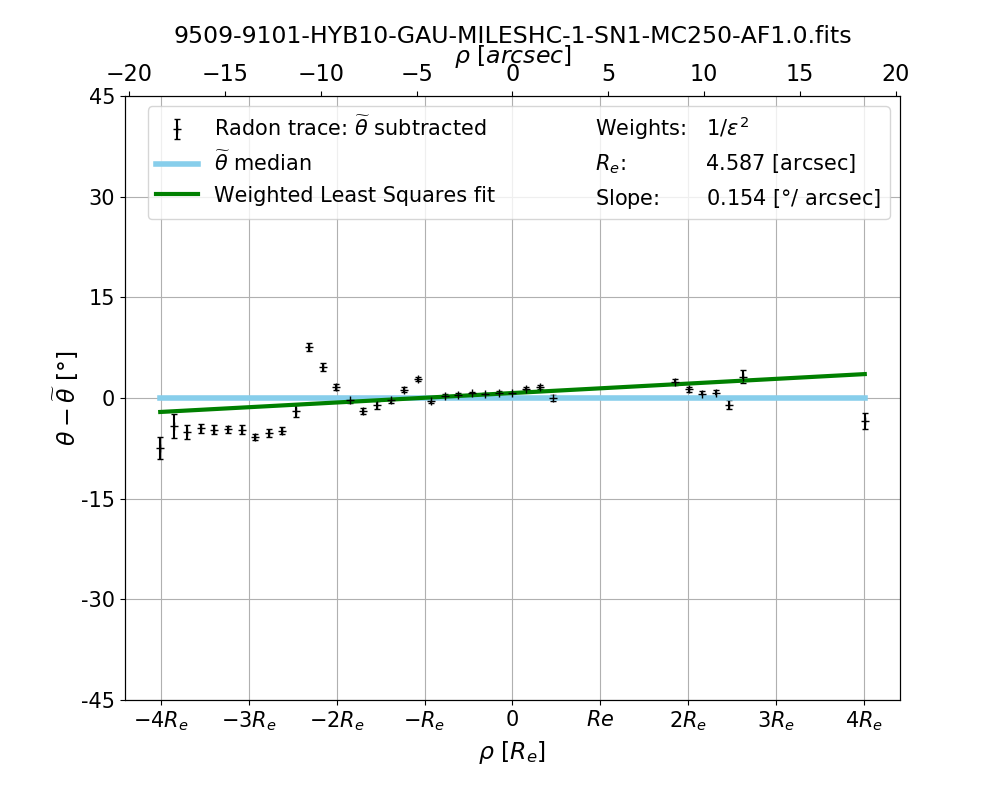
\includegraphics[width=0.31\textwidth]{Images/WLSFITS/CC0/9509-9101.png}
    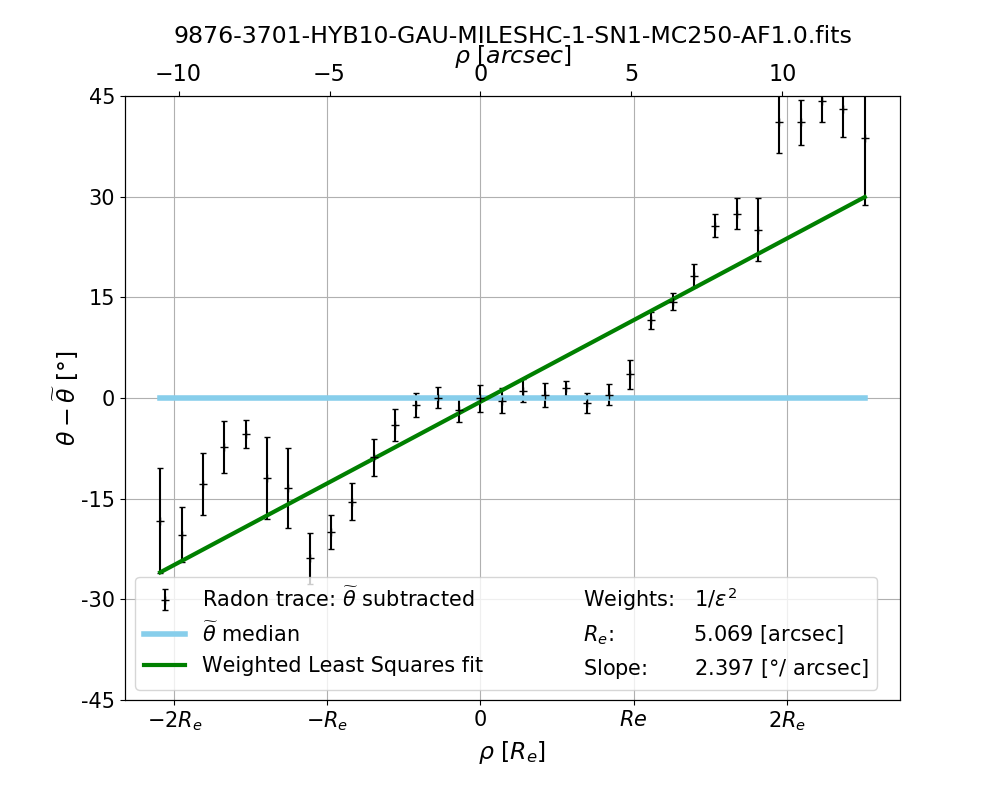
\includegraphics[width=0.31\textwidth]{Images/WLSFITS/CC0/9876-3701.png}
    %
%
    \caption{Radon transform trace plots of the control galaxy sample CC0 (set 2 0f 2). The content description is as per Figure \ref{fig:Radon-traces-CPSB-WLSFITS-1}.}
    \label{fig:Radon-traces-CC0-WLSFITS-2}
\end{figure*}

\begin{figure*}
    \centering
    \includegraphics[width=0.31\textwidth]{Images/WLSFITS/CC1/7958-3704.png}
    \includegraphics[width=0.31\textwidth]{Images/WLSFITS/CC1/7990-9102.png}
    \includegraphics[width=0.31\textwidth]{Images/WLSFITS/CC1/8131-12704.png}
    %
    \includegraphics[width=0.31\textwidth]{Images/WLSFITS/CC1/8131-6104.png}
    \includegraphics[width=0.31\textwidth]{Images/WLSFITS/CC1/8133-3701.png}
    \includegraphics[width=0.31\textwidth]{Images/WLSFITS/CC1/8241-12702.png}
    %
    \includegraphics[width=0.31\textwidth]{Images/WLSFITS/CC1/8252-1902.png}
    \includegraphics[width=0.31\textwidth]{Images/WLSFITS/CC1/8255-3704.png}
    \includegraphics[width=0.31\textwidth]{Images/WLSFITS/CC1/8456-3703.png}
    %
    \includegraphics[width=0.31\textwidth]{Images/WLSFITS/CC1/8465-1902.png}
    \includegraphics[width=0.31\textwidth]{Images/WLSFITS/CC1/8465-3703.png}
    \includegraphics[width=0.31\textwidth]{Images/WLSFITS/CC1/8465-9101.png}
    %
    \includegraphics[width=0.31\textwidth]{Images/WLSFITS/CC1/8548-6104.png}
    \includegraphics[width=0.31\textwidth]{Images/WLSFITS/CC1/8550-3701.png}
    \includegraphics[width=0.31\textwidth]{Images/WLSFITS/CC1/8591-6103.png}
%
    \caption{Radon transform trace plots of the control galaxy sample CC1 (set 1 0f 2). The content description is as per Figure \ref{fig:Radon-traces-CPSB-WLSFITS-1}.}
    \label{fig:Radon-traces-CC1-WLSFITS-1}
\end{figure*}

\begin{figure*}
    \centering
    \includegraphics[width=0.31\textwidth]{Images/WLSFITS/CC1/8601-3704.png}
    \includegraphics[width=0.31\textwidth]{Images/WLSFITS/CC1/8616-3704.png}
    \includegraphics[width=0.31\textwidth]{Images/WLSFITS/CC1/8715-6103.png}
    %
    \includegraphics[width=0.31\textwidth]{Images/WLSFITS/CC1/8940-6101.png}
    \includegraphics[width=0.31\textwidth]{Images/WLSFITS/CC1/8990-1901.png}
    \includegraphics[width=0.31\textwidth]{Images/WLSFITS/CC1/8991-3704.png}
    %
    \includegraphics[width=0.31\textwidth]{Images/WLSFITS/CC1/9002-6103.png}
    \includegraphics[width=0.31\textwidth]{Images/WLSFITS/CC1/9025-6104.png}
    \includegraphics[width=0.31\textwidth]{Images/WLSFITS/CC1/9182-12703.png}
    %
    \includegraphics[width=0.31\textwidth]{Images/WLSFITS/CC1/9184-1901.png}
    \includegraphics[width=0.31\textwidth]{Images/WLSFITS/CC1/9195-1901.png}
    \includegraphics[width=0.31\textwidth]{Images/WLSFITS/CC1/9497-12704.png}
    %
    \includegraphics[width=0.31\textwidth]{Images/WLSFITS/CC1/9508-3701.png}
    \includegraphics[width=0.31\textwidth]{Images/WLSFITS/CC1/9869-12701.png}
%
    \caption{Radon transform trace plots of the control galaxy sample CC1 (set 2 0f 2). The content description is as per Figure \ref{fig:Radon-traces-CPSB-WLSFITS-1}.}
    \label{fig:Radon-traces-CC1-WLSFITS-2}
\end{figure*}


